\chapterimage{chapter_head_2.pdf} % Chapter heading image

\chapter{Percepção musical}
\label{cap:percepcaomusical}
\begin{definition}[Percepção musical] 
\index{Musicalidade!Percepção musical}
\label{def:PercepcaoMusical}
É a capacidade de distinguir e reconhecer aspectos da música 
tais como melodias, ritmos, \hyperref[sec:texturasmusica]{\textbf{texturas}}, 
\hyperref[sec:FormaMusical]{\textbf{formas}}, 
\hyperref[sec:Frase]{\textbf{frases}}, 
%\hyperref[sec:intervalomelodico]{\textbf{intervalos}}, 
\hyperref[sec:Cadencia]{\textbf{cadências}} \cite[pp. 29]{teoriamusicala2012}, etc.
Na percepção musical são utilizadas áreas do cérebro, 
dedicadas à descomposição em frequência,
e ao processo de percepção de estruturas de tempo \cite{de2019especializacao}.
\end{definition}

\section{Caracteristicas da melodia}
\label{sec:caracteristicas:melodia}
\index{Musicalidade!Melodia}


Se descrevemos uma \hyperref[sec:pos:Melodia]{\textbf{melodia}} em função das relações existentes entre os tons,
podemos definir as seguintes caraterísticas: 
A extensão (``range'' em inglês),
o contorno  (``shape'' ou ``contour'' em inglês) e 
o movimento  (``movement'' em inglês) 
\cite[pp. 43]{holland2013music} \cite[pp. 50]{langer2017theory}.

\begin{description}
%%%%    %%%%    %%%%    %%%%    %%%%
\item[A extensão melódica:] 
\label{ref:melodica:range}
\index{Musicalidade!Extensão melódica}
Refere-se à extensão entre a nota de maior 
e a de menor \hyperref[sec:pos:Altura]{\textbf{altura}},
 numa melodia ou uma parte dela \cite[pp. 43]{holland2013music}.

\begin{example}[Extensão de uma melodia]
Na pauta descrita na Figura \ref{fig:melody:range:1}, 
vemos uma melodia com uma extensão de 11 semitons, pois a nota mais grave é um dó,
e a mais aguda um si.

Por outro lado se só analisamos uma porção dela, como os 2 primeiros compassos,
então a extensão seria de 7 semitons, pois a nota mais grave é um dó e a mais aguda um sol.
\end{example}
\begin{figure}[!h]
\centering
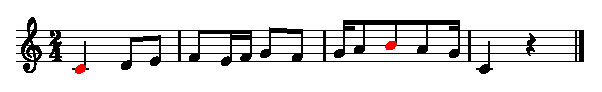
\includegraphics[width=0.99\textwidth]{chapters/cap-musicalidade-percepcion/melodia-carateristicas-range.eps}
\caption{Rango da melodia.}
\label{fig:melody:range:1}
\end{figure}

Subjetivamente falando, geralmente, as extensões provocam em nós as seguintes reações:
\begin{itemize}
\item Melodias com uma extensão pequena, nos produzem geralmente um clima de calma ou quietude
 \cite[pp. 43]{holland2013music}.
\item Melodias com extensões maiores, nos produzem geralmente uma sensação de liberdade e expansividade
 \cite[pp. 43]{holland2013music}.
\end{itemize}

%%%%    %%%%    %%%%    %%%%    %%%%
\item[O contorno melódico:] 
\label{ref:melodica:shape}
\index{Musicalidade!Contorno melódico}
Refere-se ao contorno criado pelas mudanças de altura de uma melodia,
podemos imaginar ao contorno como uma linha formada pelas cabeças das notas musicais 
\cite[pp. 44]{holland2013music} \cite[pp. 61]{chazin2016teaching} \cite[pp. 50]{langer2017theory},
como quando unimos pontos para formar um desenho num livro infantil.


\begin{example}[Contorno de uma melodia]
Se usamos a melodia descrita na Figura \ref{fig:melody:range:1}, 
o contorno da melodia é descrito pela linha que une as cabeças das figuras musicais,
como mostra a Figura \ref{fig:melody:shape:1}.
\end{example}
\begin{figure}[!h]
\centering
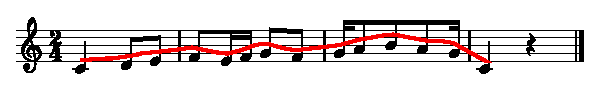
\includegraphics[width=0.99\textwidth]{chapters/cap-musicalidade-percepcion/melodia-carateristicas-shape.eps}
\caption{Contorno da melodia.}
\label{fig:melody:shape:1}
\end{figure}

Para um dançarino é importante reconhecer o contorno de uma melodia, 
pois assim este pode discernir o \hyperref[ref:climax]{\textbf{clímax}} de cada frase musical, 
e perceber como estas se relacionam com as outras frases musicais
\cite[pp. 45]{holland2013music}.

%%%%    %%%%    %%%%    %%%%    %%%%
\item[O movimento melódico:]
\label{ref:melodica:movimento}
O termo movimento se refere à distancia relativa entre as notas consecutivas de uma melodia;
onde os movimentos melódicos podem ser categorizados como conjuntos ou disjuntos 
\cite[pp. 52]{langer2017theory} \cite[pp. 165]{reinato2010musicavol1} \cite[pp. 45]{holland2013music}. 
\begin{itemize}
\item Um \textbf{movimento melódico conjunto} indica 
\label{ref:melodica:movimento:conjunto}
que as figuras musicais consecutivas
tem sempre \hyperref[sec:intervalomelodico]{\textbf{intervalos}} consecutivos,
ascendentes ou descendentes; estes podem ser intervalos de 
\hyperref[tab:intervalomelodico2]{\textbf{segunda menor}},
\hyperref[tab:intervalomelodico2]{\textbf{segunda maior}} e
os cromáticos  \cite[pp. 165]{reinato2010musicavol1} \cite[pp. 52]{langer2017theory}.  
\item Um \textbf{movimento melódico disjunto} indica 
\label{ref:melodica:movimento:disjunto}
que as figuras musicais consecutivas
se movimentam em \hyperref[sec:intervalomelodico]{\textbf{intervalos}} 
de \hyperref[tab:intervalomelodico2]{\textbf{terça menor}} ou superiores 
\cite[pp. 166]{reinato2010musicavol1} \cite[pp. 53]{langer2017theory}.
\end{itemize}~

\begin{example}[Movimento de uma melodia]
Se usamos a melodia descrita na Figura \ref{fig:melody:range:1},
observamos que esta é conjunta na maior parte dela,
excepto na transição entre o terceiro e quarto compasso,
onde o movimento é disjunto,
como mostra a Figura \ref{fig:melody:movement:1}.
\end{example}
\begin{figure}[!h]
\centering
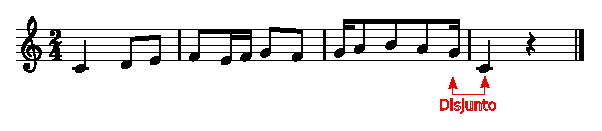
\includegraphics[width=0.99\textwidth]{chapters/cap-musicalidade-percepcion/melodia-carateristicas-movement.eps}
\caption{Movimento da melodia.}
\label{fig:melody:movement:1}
\end{figure}

As melodias tendem a ser compostas de forma conjunta, 
pois desse jeito são mais fáceis de cantar,
e dependendo do instrumento musical, mais fáceis de executar  
\cite[pp. 53]{langer2017theory}. 

\end{description}~


\PRLsep{Treinamentos}


\begin{example}[Treinamento para reconhecer o contorno melódico:]
Um bom treinamento de percepção melódica,
para que nossa mente esteja preparada para perceber o contorno melódico,
seria escutar de forma aleatória\footnote{Para conseguir a escolha aleatória,
você pode colocar as musicas numa playlist que execute as músicas 
seguindo algum algoritmo pseudoaleatório;
ou também pode pedir a algum amigo que selecione as melodias enquanto você tenta reconhecê-la,
esta forma tem a vantagem que se você não consegue reconhecer na primeira tentativa,
pode pedir a ele repetir a melodia.} 
as melodias que produzem as pautas da Figura \ref{fig:9melodias},
e tentar reconhecer a qual pauta pertencem só pela nossa audição.
\end{example}


\begin{example}[Treinamento para reconhecer a extensão melódica:]
Usando as  pautas mostradas na Figura \ref{fig:9melodias},
poderíamos treinar nossa percepção da extensão melódica,
e tentar reconhecer, escolhendo aleatoriamente as melodias, 
se estas tem uma extensão pequena ou grande.

Além desse treinamento, podemos tentar deduzir qual é a nota musical de menor tom, 
e qual é a de maior tom.
\end{example}


\begin{figure}[!h]
     \centering
     %%%
     \begin{subfigure}[b]{0.3\textwidth}
         \centering
         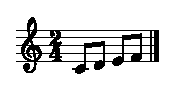
\includegraphics[width=\textwidth]{chapters/cap-musicalidade-percepcion/melodia-chars-shape-1-1.eps}
         \caption{Melodia 1.}
         \label{fig:melodia-chars-shape-1-1}
     \end{subfigure}
     \hfill
     %%%
     \begin{subfigure}[b]{0.3\textwidth}
         \centering
         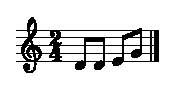
\includegraphics[width=\textwidth]{chapters/cap-musicalidade-percepcion/melodia-chars-shape-2-1.eps}
         \caption{Melodia 2.}
         \label{fig:melodia-chars-shape-2-1}
     \end{subfigure}
     \hfill
     %%%
     \begin{subfigure}[b]{0.3\textwidth}
         \centering
         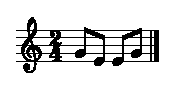
\includegraphics[width=\textwidth]{chapters/cap-musicalidade-percepcion/melodia-chars-shape-3-1.eps}
         \caption{Melodia 3.}
         \label{fig:melodia-chars-shape-3-1}
     \end{subfigure}
     \hfill
     %%%
     \begin{subfigure}[b]{0.3\textwidth}
         \centering
         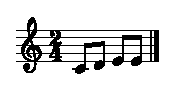
\includegraphics[width=\textwidth]{chapters/cap-musicalidade-percepcion/melodia-chars-shape-4-1.eps}
         \caption{Melodia 4.}
         \label{fig:melodia-chars-shape-4-1}
     \end{subfigure}
     \hfill
     %%%
     \begin{subfigure}[b]{0.3\textwidth}
         \centering
         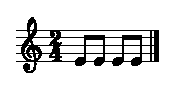
\includegraphics[width=\textwidth]{chapters/cap-musicalidade-percepcion/melodia-chars-shape-5-1.eps}
         \caption{Melodia 5.}
         \label{fig:melodia-chars-shape-5-1}
     \end{subfigure}
     \hfill
     %%%
     \begin{subfigure}[b]{0.3\textwidth}
         \centering
         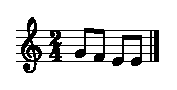
\includegraphics[width=\textwidth]{chapters/cap-musicalidade-percepcion/melodia-chars-shape-6-1.eps}
         \caption{Melodia 6.}
         \label{fig:melodia-chars-shape-6-1}
     \end{subfigure}
     \hfill
     %%%
     \begin{subfigure}[b]{0.3\textwidth}
         \centering
         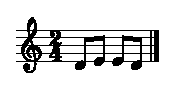
\includegraphics[width=\textwidth]{chapters/cap-musicalidade-percepcion/melodia-chars-shape-7-1.eps}
         \caption{Melodia 7.}
         \label{fig:melodia-chars-shape-7-1}
     \end{subfigure}
     \hfill
     %%%
     \begin{subfigure}[b]{0.3\textwidth}
         \centering
         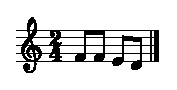
\includegraphics[width=\textwidth]{chapters/cap-musicalidade-percepcion/melodia-chars-shape-8-1.eps}
         \caption{Melodia 8.}
         \label{fig:melodia-chars-shape-8-1}
     \end{subfigure}
     \hfill
     %%%
     \begin{subfigure}[b]{0.3\textwidth}
         \centering
         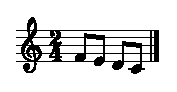
\includegraphics[width=\textwidth]{chapters/cap-musicalidade-percepcion/melodia-chars-shape-9-1.eps}
         \caption{Melodia 9.}
         \label{fig:melodia-chars-shape-9-1}
     \end{subfigure}
     \hfill
        \caption{Tipos de contornos melódicos}
        \label{fig:9melodias}
\end{figure}




\newpage

\section{Texturas na música}
\index{Música!Texturas}
\label{sec:texturasmusica}
\begin{wrapfigure}{r}{0.33\textwidth}
    \centering 
    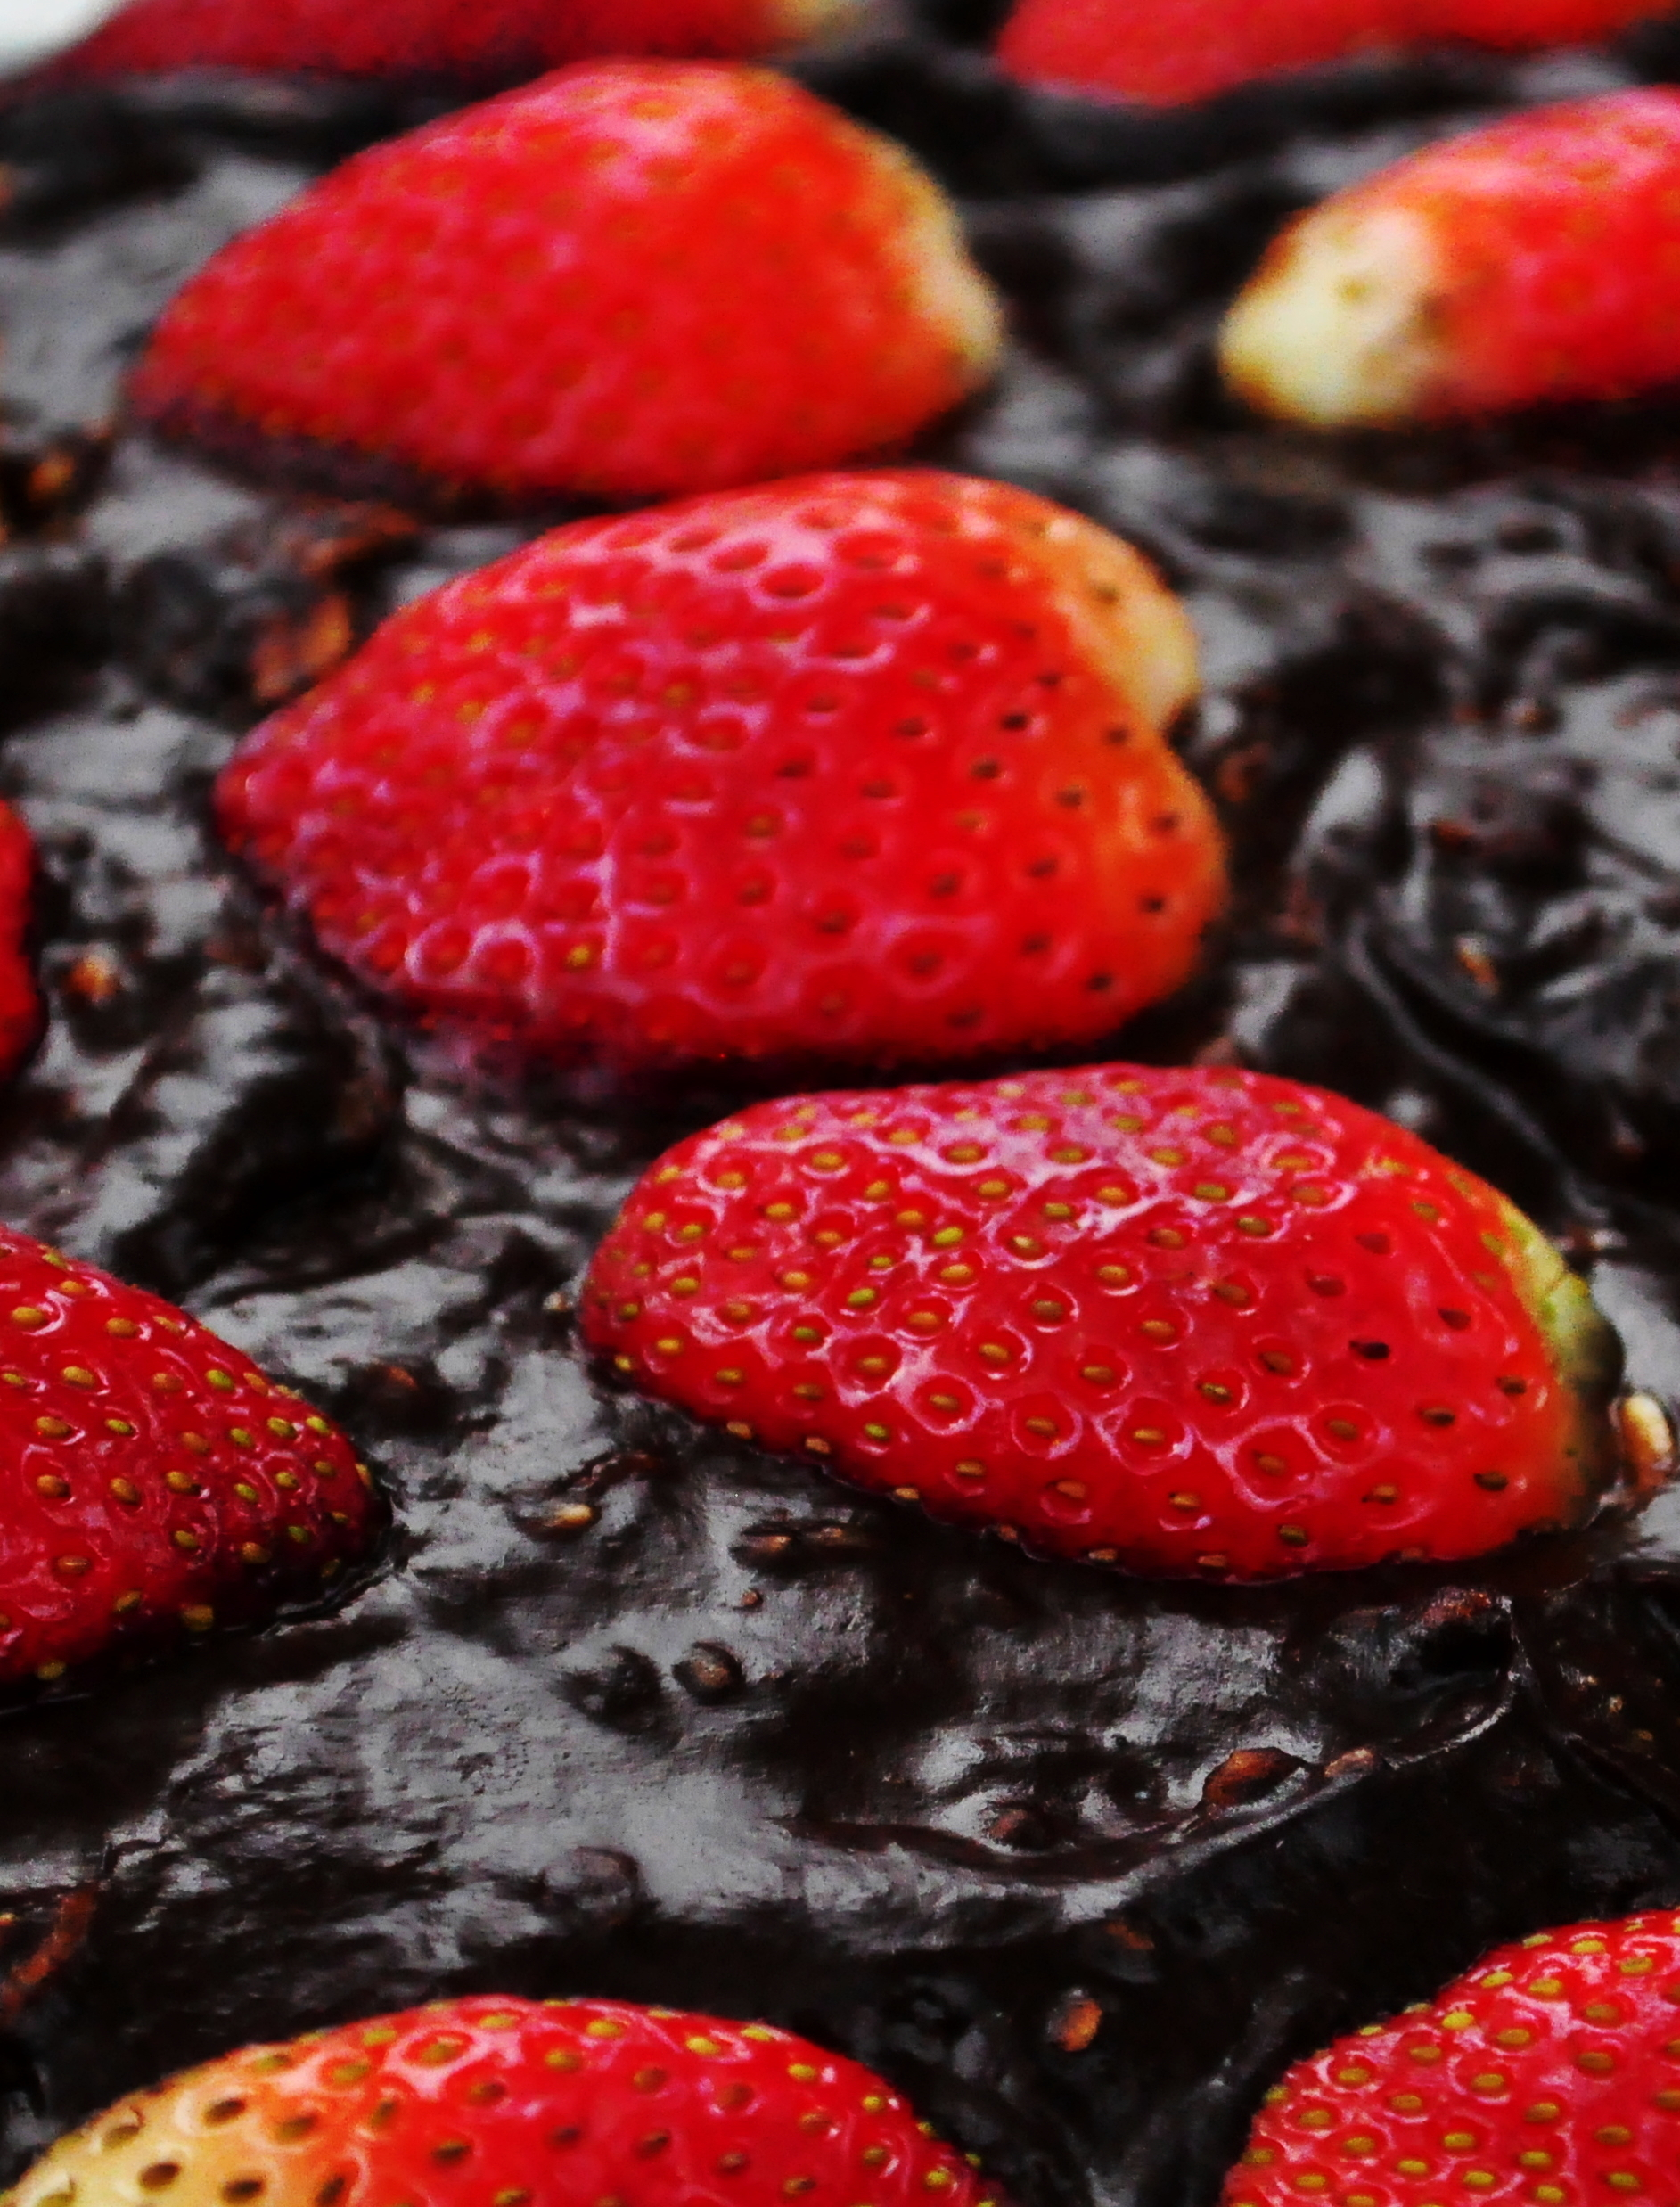
\includegraphics[width=0.30\textwidth]{chapters/cap-musicalidade-percepcion/textura.jpg}
  \caption{Texturas.}
\end{wrapfigure}
De forma similar a como descrevemos a textura numa superfície,
podemos explicar a textura na música.
A textura musical é um termo usado para indicar o modo em que interagem e 
se misturam várias linhas melódicas \cite[pp. 29]{kerman2015listen}.


O termo textura usado na música, 
implica que esta é composta por instrumentos com a capacidade de gerar tons,
e consequentemente melodias;
dado que a percussão não é geralmente considerada como melódica, 
esta não é tomada em conta quando usamos o termo textura \cite[pp. 59]{holland2013music}.

Na música atual existem  vários tipos de texturas, 
porém 3 destes tipos  são os mais comuns 
\cite[pp. 77]{copland1974ouvir} \cite[pp. 29]{kerman2015listen} \cite[pp. 322]{harnum2009basic}:
\begin{itemize}
\item textura monofônica, 
\item textura homofônica e
\item textura polifônica.
\end{itemize}

 
%%%%%%%%%%%%%%%%%%%%%%%%%%%%%%%%%%%%%%%%%%%%%%%%%%%%%%%%%%%%%%%%%%%%%%%%%%%%%%%%
\subsection{A textura monofônica}
\label{subsec:monofonica}
\index{Música!Monofônica}
\begin{wrapfigure}{r}{0.33\textwidth}
\centering
    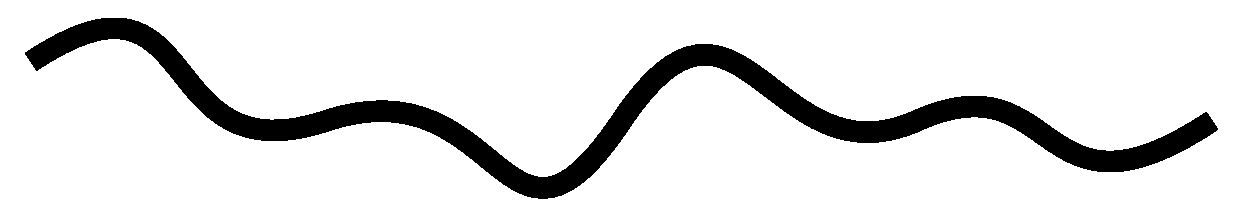
\includegraphics[width=0.31\textwidth]{chapters/cap-musicalidade-percepcion/monofonica1.eps}
  \caption{Textura monofônica.}
\end{wrapfigure}
Este tipo de música tem uma única linha melódica sem acompanhamento.
Consequentemente este tipo de música é a mais simples de ouvir, 
pois nossa atenção cai sobre uma única camada na música \cite[pp. 77]{copland1974ouvir} \cite[pp. 29]{kerman2015listen}.
A música monofônica corresponde ao tipo mais antigo de música \cite[pp. 539]{apel1969harvard}.

Se considera que é uma textura monofônica, mesmo que sejam muitas vozes as que executem uma mesma melodia, 
ou que estas executem a mesma melodia em oitavas diferentes \cite[pp. 42]{bennett1993elementos} \cite[pp. 58]{holland2013music}.

A qualificação de textura  monofônica não é afetada pelo uso de instrumentos de percussão tocando junto com a melodia;
a textura monofônica refere-se à parte tonal da música, é dizer à melodia, 
não à textura rítmica da música \cite[pp. 58]{holland2013music}.

\begin{example}
A Figura \ref{fig:ex:monofonica} mostra um exemplo de uma seção de música com textura monofônica.
\end{example}

\begin{figure}[!h]
\centering
    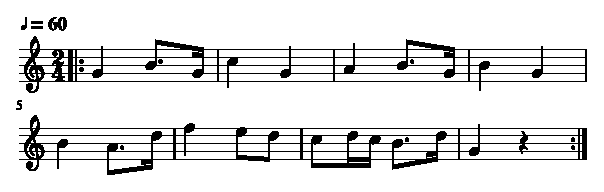
\includegraphics[width=0.99\textwidth]{chapters/cap-musicalidade-percepcion/textura-monofonica-1.eps}
  \caption{Textura monofônica.}
\label{fig:ex:monofonica}
\end{figure}
 
\begin{example}
Um exemplo, no ocidente,  muito depurado de música monofônica é o canto gregoriano
\cite[pp. 77]{copland1974ouvir} \cite[pp. 29]{kerman2015listen} \cite[pp. 58]{holland2013music}. 
Aqui, não importa o número de vozes usadas na interpretação,
pois todas seguem a mesma linha melódica, pelo que é considerada uma textura monofônica.
\end{example}

%monodia \cite[pp. 38]{schurmann1989m} 

%%%%%%%%%%%%%%%%%%%%%%%%%%%%%%%%%%%%%%%%%%%%%%%%%%%%%%%%%%%%%%%%%%%%%%%%%%%%%%%%
\subsection{A textura homofônica}
\label{subsec:homofonica}
\index{Música!Honofônica}
\begin{wrapfigure}{r}{0.33\textwidth}
  \centering
    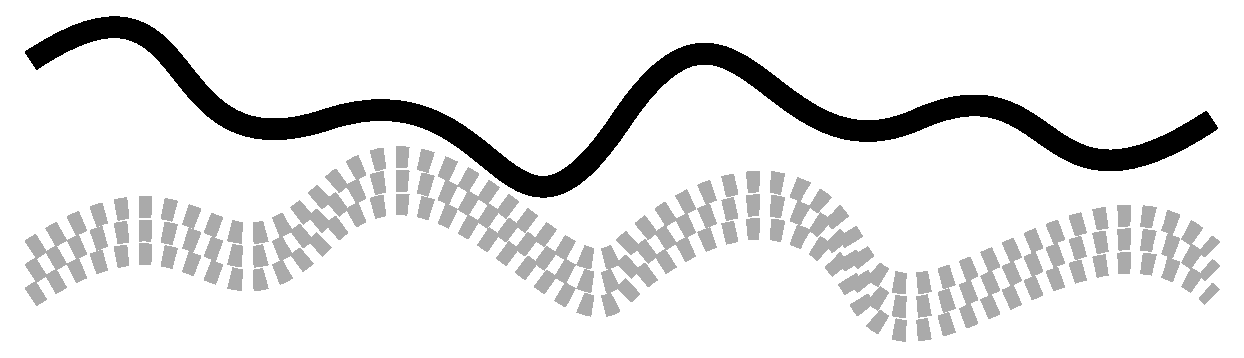
\includegraphics[width=0.31\textwidth]{chapters/cap-musicalidade-percepcion/honofonica1.eps}
  \caption{Textura homofônica.}
\end{wrapfigure}
O termo ``homofônico'' ou ``homofonia'' significa literalmente ``vozes semelhantes''.%% Falta referença
A textura homofônica consiste de uma linha melódica principal e um acompanhamento por acordes,
de modo que existe uma distinção clara entre a melodia e a harmonia de acompanhamento;
esta textura é o tipo  mais usado na música atual,
e só é ligeiramente mais complexa que a textura monofônica 
\cite[pp. 78]{copland1974ouvir} \cite[pp. 29]{kerman2015listen} 
\cite[pp. 43]{bennett1993elementos} \cite[pp. 58]{holland2013music}.


A homofonia é o oposto da polifonia, 
pois na textura homofônica só uma linha melódica é importante,
enquanto que na textura polifônica todas as partes contribuem equitativamente para gerar o tecido musical
\cite[pp. 687]{apel1969harvard}.

\begin{example}
A Figura \ref{fig:ex:homofonica} mostra um exemplo de uma seção de musica com textura homofônica.
\end{example}

\begin{figure}[!h]
\centering
    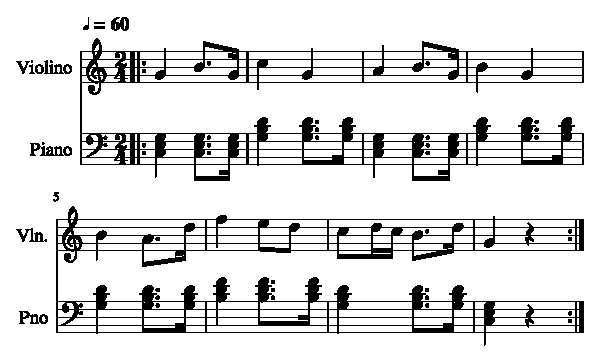
\includegraphics[width=0.99\textwidth]{chapters/cap-musicalidade-percepcion/textura-homofonica-1.eps}
  \caption{Textura homofônica.}
\label{fig:ex:homofonica}
\end{figure}

\begin{example}
Um exemplo de textura homofônica pode ser visto no choro ``Deixe o breque pra mim'',
de Altamiro Carrilho, 
onde a melodia principal é feita por um único instrumento (flauta), 
com uma base harmônica e percussiva, de acompanhamento.
\end{example}

%\cite[pp. 121]{schurmann1989m} 


%%%%%%%%%%%%%%%%%%%%%%%%%%%%%%%%%%%%%%%%%%%%%%%%%%%%%%%%%%%%%%%%%%%%%%%%%%%%%%%%
\subsection{A textura polifônica}
\index{Música!Polifônica}
\label{subsec:polifonica}
\begin{wrapfigure}{r}{0.33\textwidth}
\centering
    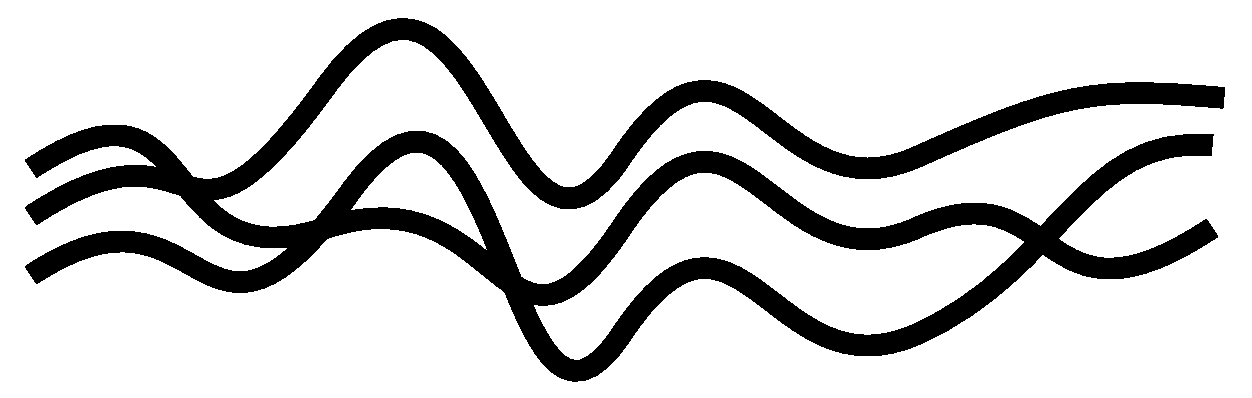
\includegraphics[width=0.31\textwidth]{chapters/cap-musicalidade-percepcion/polifonica1.eps}
  \caption{Textura polifônica.}
\end{wrapfigure}
Termo proveniente do grego, que significa ``vozes múltiplas''.%% Falta referença
A música com textura polifônica se carateriza por ter duas ou mais linhas melódicas, 
que se entrelaçam continuamente;
as melodias são consideradas independentes e de interesse aproximadamente igual.
A percepção da música polifônica precisa de um maior nível de atenção, 
em comparação das texturas monofônica e homofônica,
pois exige ao ouvinte a capacidade de separar mentalmente cada linha melódica  
\cite[pp. 79-80]{copland1974ouvir} \cite[pp. 29]{kerman2015listen} 
\cite[pp. 42]{bennett1993elementos} \cite[pp. 59]{holland2013music}
\cite[pp. 687]{apel1969harvard}.

Uma termo frequentemente usado na música polifônica é o contraponto;
que é a técnica de escrever duas ou mais melodias que se encaixam 
\cite[pp. 29]{kerman2015listen} \cite[pp. 42]{bennett1993elementos}.

\begin{tcbinformation} 
\label{ref:quantasvozes}
\textbf{Quantas vozes independentes pode captar simultaneamente um ser humano?}
Não existe um senso comum, porém pode-se afirmar que treinando um pouco,
é possível perceber independentemente 2 ou 3 vozes sendo executadas em simultâneo \cite[pp. 81]{copland1974ouvir}. 
\end{tcbinformation} 

\begin{example}
Um exemplo de textura homofônica pode ser visto na música ``Canto e Contraponto'',
de Toquinho e Vinícius, 
onde temos uma melodia executada pela voz, e outra melodia executada por um instrumento fazendo o contraponto, 
com uma base harmônica de acompanhamento.
\end{example}

\begin{example}
A Figura \ref{fig:ex:polifonica} mostra um exemplo de uma seção de musica com textura polifônica.
\end{example}

\begin{figure}[!h]
\centering
    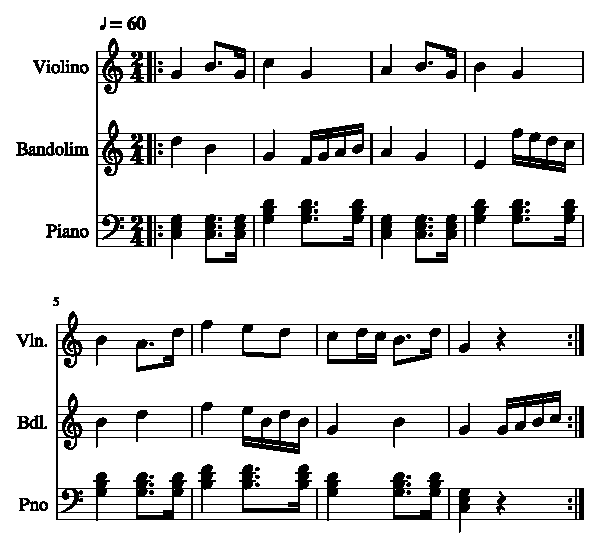
\includegraphics[width=0.99\textwidth]{chapters/cap-musicalidade-percepcion/textura-polifonica-1.eps}
  \caption{Textura polifônica.}
\label{fig:ex:polifonica}
\end{figure}



%\cite[pp. 64]{schurmann1989m} 

%%%%%%%%%%%%%%%%%%%%%%%%%%%%%%%%%%%%%%%%%%%%%%%%%%%%%%%%%%%%%%%%%%%%%%%%%%%%%%%%
\subsubsection{Polirritmia}
\index{Música!Polirritmia}
\label{subsec:polirritmia}
A polirritmia é a superposição de dois ou mais ritmos.
A polirritmia acontece quando se executam musicas com texturas polifônicas ou homofônicas
\cite[pp. 93]{alves2004teoria};
ou quando vários instrumentos de percussão tocam ritmos diferentes simultaneamente \cite[pp. 35]{holland2013music}.
Assim, a textura dos ritmos simultâneos é chamada polirritmia \cite[pp. 35]{holland2013music}.

Cada instrumento de percussão ``fala'' um ritmo único que geralmente guia os passos e movimentos dos dançarinos;
por exemplo, a música africana é conhecida por ter múltiplas camadas de ritmo e sincopas,
 que são usadas continuamente pelos dançarinos \cite[pp. 35]{holland2013music}.


É possível distinguir dois tipos de polirritmia \cite[pp. 687]{apel1969harvard}:
\begin{itemize}
\item Ritmos contrastantes dentro da mesma \hyperref[def:Metrica]{\textbf{métrica}};
por exemplo, os ritmos mostrados na Figura \ref{fig:polirritmia1-1}.
\begin{figure}[!h]
\centering
    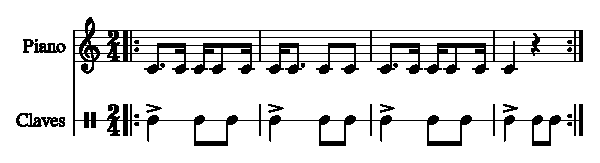
\includegraphics[width=\textwidth]{chapters/cap-musicalidade-percepcion/polirritmia1-1.eps}
  \caption{Textura polirrítmica com a mesma métrica.}
\label{fig:polirritmia1-1}
\end{figure}
\item Ritmos contrastantes com diferente \hyperref[def:Metrica]{\textbf{métrica}} ou acentuações, 
às vezes é denominado ``polimétrico'';
por exemplo, os ritmos mostrados na Figura \ref{fig:polirritmia2-1}.
\begin{figure}[!h]
\centering
    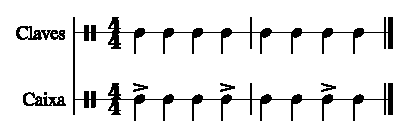
\includegraphics[width=0.7\textwidth]{chapters/cap-musicalidade-percepcion/polirritmia2-1.eps}
  \caption{Textura polirrítmica com diferente métrica.}
\label{fig:polirritmia2-1}
\end{figure}
\end{itemize}




%%%%%%%%%%%%%%%%%%%%%%%%%%%%%%%%%%%%%%%%%%%%%%%%%%%%%%%%%%%%%%%%%%%%%%%%%%%%%%%%
\section{Percepção da métrica na música}
\label{sec:percepcionmetrica}
Como foi explicado na Pag. \pageref{def:Metrica}, 
a \hyperref[def:Metrica]{\textbf{métrica}} é um padrão ordenado de \hyperref[sec:Tempo]{\textbf{tempos}} fortes e fracos,
sobre a qual a música ou uma porção dela é organizada, 
sendo o \hyperref[def:Compasso]{\textbf{compasso}} uma agrupação métrica completa.
Quando escutamos uma música e procuramos dançar-lha, 
uma caraterista importante que nos auxiliará neste objetivo,
é conhecer a métrica com que a música foi organizada.
A informação proporcionada pela métrica nos servirá de bússola;
pois conhecer quando acontecerá um tempo forte, 
e quantos tempos fracos teremos que esperar ate repetir o ciclo,
nos dará liberdade na dança para sairmos dos padrões, criar movimentos, deixar-nos levar pela imaginação ou simplesmente errar,
 e ter a confiança de que saberemos como voltar com seguridade a estar em comunião com a música;
pois em todo momento poderemos deduzir quando o ciclo, imposto pela métrica, será reiniciado.

Quando um dançarino conhece a métrica de uma música,
e consequentemente quando acontecerá o tempo forte,
este pode usar esse dado para  organizar ou predizer seus futuros movimentos, 
por exemplo:
\begin{itemize}
\item Podemos usar o tempo forte como o inicio de nossos movimentos apos uma pausa,  
intersetando esta informação com o inicio de uma \hyperref[sec:Frase]{\textbf{frase}} musical.
\item Podemos predizer os \hyperref[subsec:FinalAbertoFechado]{\textbf{finais fechados}} 
de frases musicais,
 pois geralmente estão colocados em tempos fortes.
\item Podemos calcular os breques na música, que geralmente  acontecem depois de uma frase que finaliza em tempo forte.
\item Podemos obter o \hyperref[sec:Andamento]{\textbf{andamento}} da música,
para souber a que velocidade dançaremos. 
\item Se perdemos o passo, podemos usar o tempo forte como guia para colocar-nos em sincronia com nosso par de dança.
\item etc.
\end{itemize}

Assim, é muito importante conhecer a métrica da música que estamos dançando;
porém, conhecer esta informação só escutando a música, requer um pouco de prática,
 técnica ou também sensibilidade.

Podemos abordar o problema de reconhecer a métrica seguindo dois procedimentos:
\begin{itemize}
\item \textbf{Método quase-objetivo:} Neste método, primeiro
\begin{itemize} 
\item localizaremos o tempo forte, seguindo as recomendações explicadas na Seção \ref{subsec:perceberTF1},
e posteriormente 
\item reconheceremos o tipo de compasso, 
encaixando seus tempos e distintos tipos de acentos no ciclo da métrica, 
como explicado na Seção \ref{subsec:pertipodecompasso};
\end{itemize}
todo este procedimento é descrito no diagrama de fluxo mostrado na Figura \ref{fig:fluxodancanopulso1}.

Este método tem sido catalogado como quase-objetivo,
porque mesmo que detetar o tempo forte seja um método com bastante ``técnica'',
detetar o tipo de compasso pode precisar um ligeiro nível de ``sensibilidade'' ou treino
para perceber se os acentos, do tipo de compasso proposto, batem com a música analisada. 
\item \textbf{Método quase-subjetivo:} Neste método, primeiro 
\begin{itemize}
\item reconheceremos o \hyperref[ref:Pulso]{\textbf{pulso}} da música, como explicado na Seção \ref{subsec:perpulsomusica};
e posteriormente 
\item localizaremos entre os pulsos ao tempo forte, 
seguindo as recomendações explicadas na Seção \ref{subsec:perceberTF1},
obtendo assim a localização do tempo forte e dos tempos fracos, e consequentemente conheceremos a métrica;
\end{itemize}
todo este procedimento é descrito no diagrama de fluxo mostrado na Figura \ref{fig:fluxodancanopulso2}.

Este método tem sido catalogado como quase-subjetivo,
porque a detecção do pulso requer de  ``sensibilidade'' à música ou treino,
e mesmo que detetar o tempo forte seja um método com bastante ``técnica'',
para chegar a este ponto primeiro devemos estar seguros que detetamos bem o pulso,
pelo que a principio algumas pessoas, com pouca sensibilidade a música, podem ter problemas com este método.
\end{itemize}

\begin{figure}[h]
    \centering 
\begin{subfigure}[c]{0.45\textwidth}
\centering 
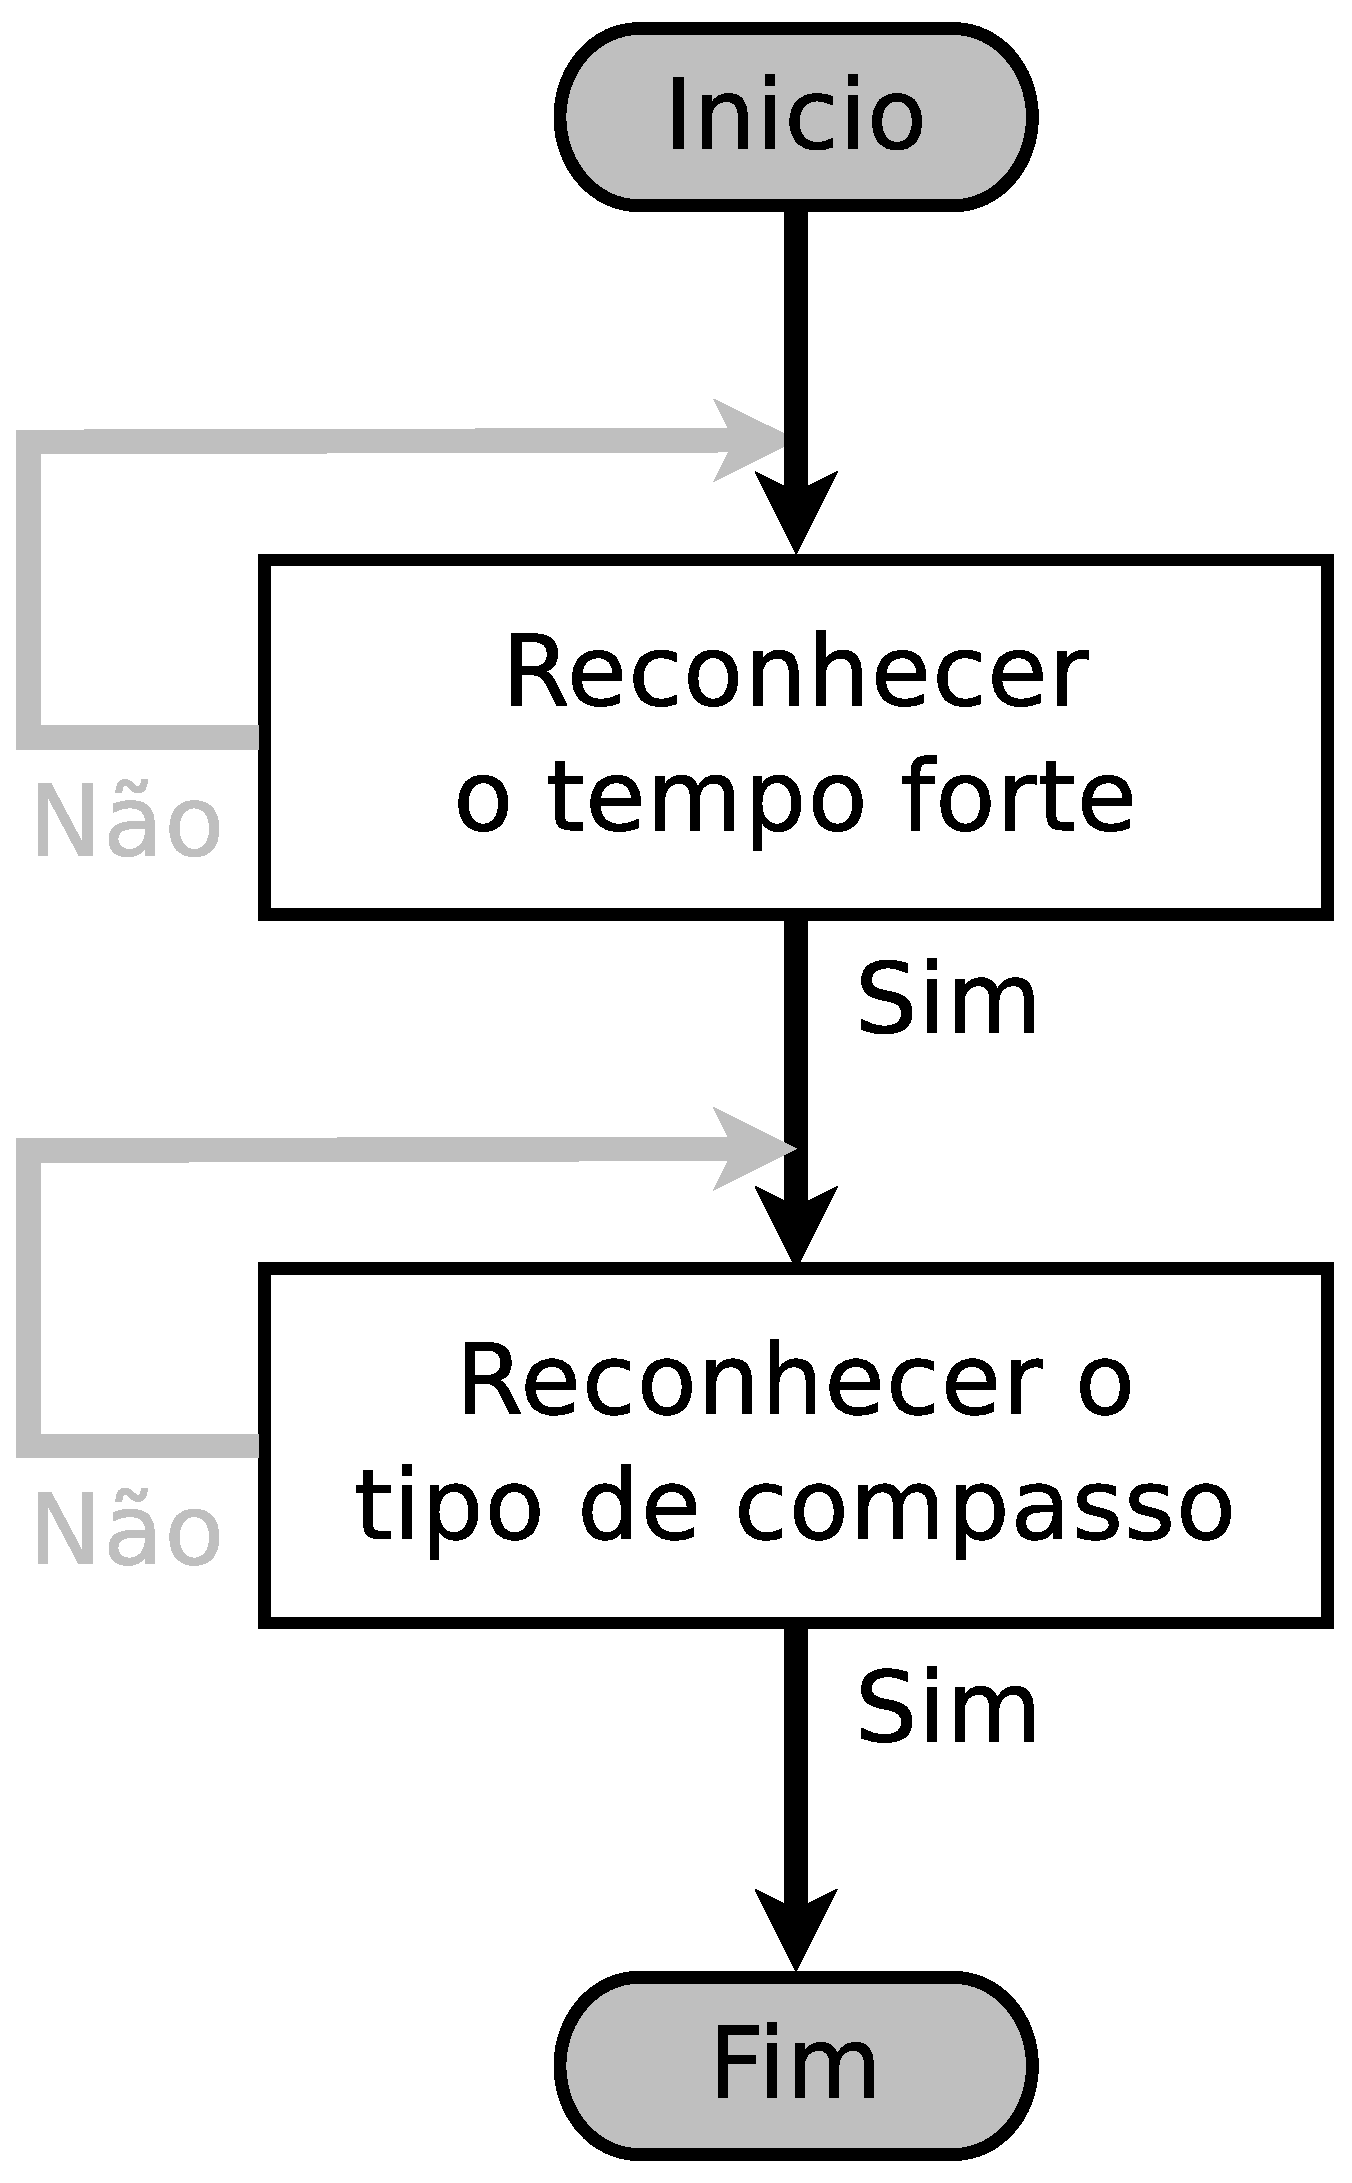
\includegraphics[width=0.65\textwidth]{chapters/cap-musicalidade-percepcion/dancanopulso1.eps}
\caption{Método quase-objetivo.}
\label{fig:fluxodancanopulso1}
\end{subfigure}
~%
\begin{subfigure}[c]{0.45\textwidth}
\centering 
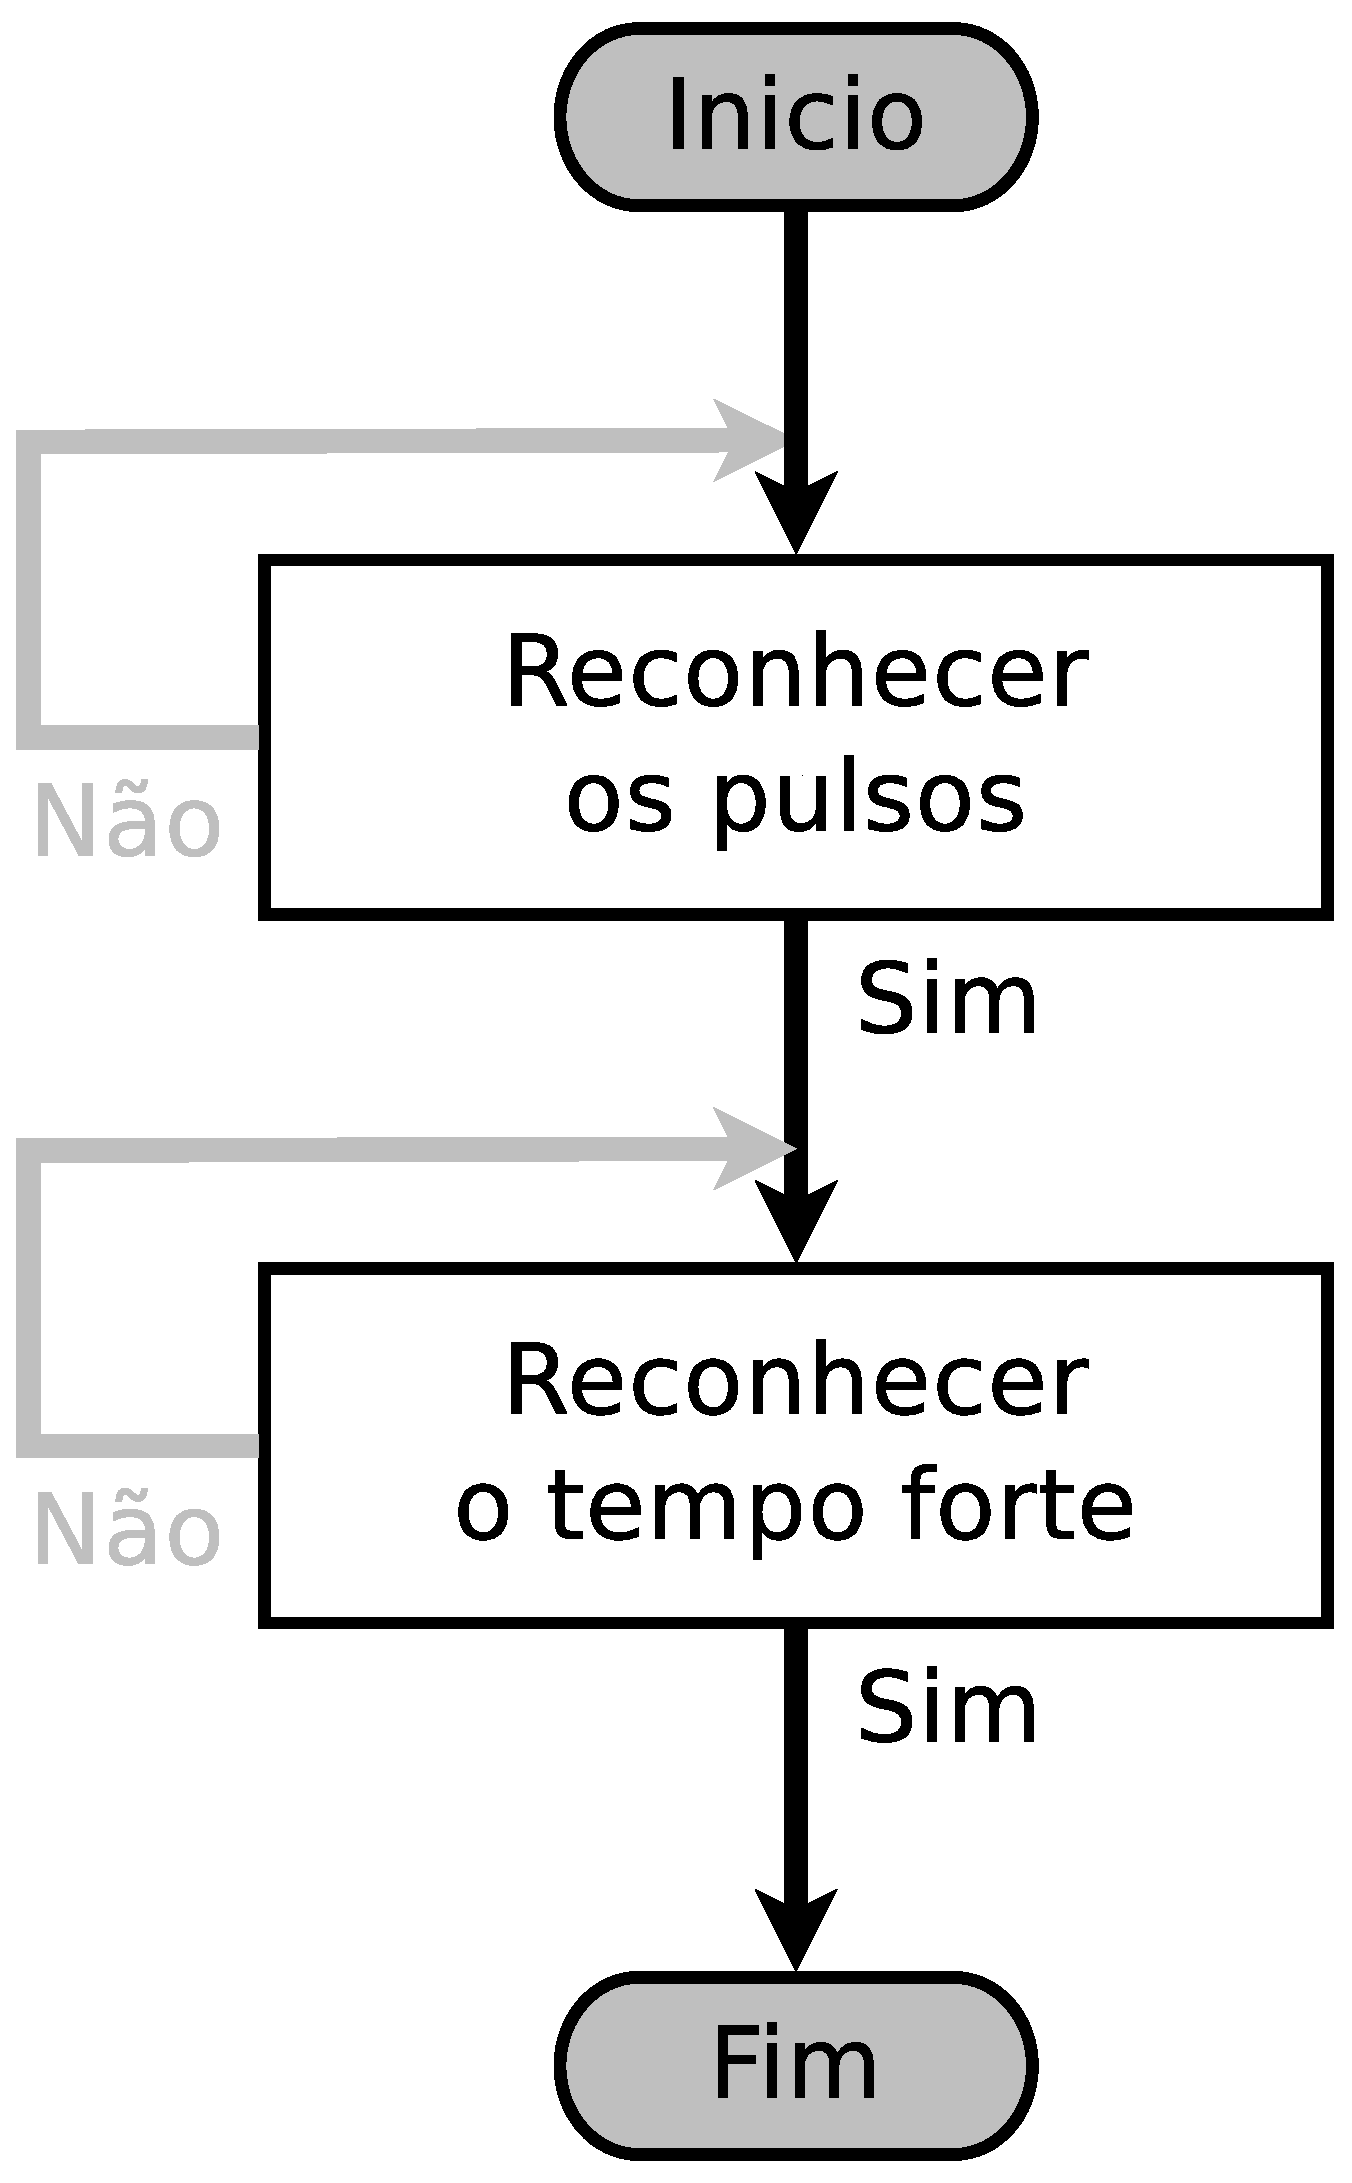
\includegraphics[width=0.65\textwidth]{chapters/cap-musicalidade-percepcion/dancanopulso2.eps}
\caption{Método quase-subjetivo}
\label{fig:fluxodancanopulso2}
\end{subfigure}
    \caption{Percebendo a métrica de uma música}\label{fig:fluxodancanopulso}
\end{figure}



%%%%%%%%%%%%%%%%%%%%%%%%%%%%%%%%%%%%%%%%%%%%%%%%%%%%%%%%%%%%%%%%%%%%%%%%%%%%%%%%
\subsection{Reconhecer o pulso}
\index{Musicalidade!Percepção do pulso}
\label{subsec:perpulsomusica}
As pessoas tendemos a dar palmas ou pisar com o pé, para acompanhar o ritmo da música como um todo,
isto acontece porque inconscientemente percebemos nela um batimento,
continuo e regular, como os batimentos do coração;
assim, quando damos palmas para acompanhar à música, o que estamos 
fazendo e reconhecer o  \hyperref[ref:Pulso]{\textbf{pulso}} musical. 

Este ato está vinculado mais a uma sensação que a um raciocínio,
pelo que é difícil apontar um método para reconhecer o pulso,
que não seja simplesmente indicar que debemos bater palmas ate ``sentir'',
que o pulso das palmas acompanhe ao pulso da música\footnote{Uma
sugestão é fazer isto fechando os olhos para evitar distrações e agudizar os outros sentidos. }.

Porém, sim podemos apontar alguns motivos que inconscientemente nos provocam chegar a este estado de sincronia.
Por exemplo, na Figura \ref{ritmo:procurando-pulso1},
\begin{figure}[!h]
\centering
    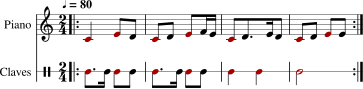
\includegraphics[width=\textwidth]{chapters/cap-musicalidade-percepcion/procurando-pulso1-1.eps}
\caption{Melodia e percussão.}
\label{ritmo:procurando-pulso1}
\end{figure}
podemos ver uma melodia acompanhada por uma percussão,
sendo ``piano'' e ``claves'' escritas usando  \hyperref[subsec:compassobinario]{\textbf{compassos binários}}, 
é dizer com dois tempos, um forte e um fraco, equivalentes cada um à duração de um \hyperref[ref:Pulso]{\textbf{pulso}}.
Assim, se nós fazemos a experiencia de escutar a música descrita na Figura \ref{ritmo:procurando-pulso1},
``sentiremos'' que podemos dar palmas ate sincroniza-nos com o pulso da música\footnote{Oito
palmas em total ate que a música seja reiniciada.}.
Isto é possível, 
a pesar de que em ambos casos as \hyperref[sec:figurasmusicais]{\textbf{figuras musicais}} usadas tem na sua maioria
\hyperref[sec:pos:Duracion]{\textbf{durações}} menores a um tempo;
podemos ver também o uso em menor quantidade de figuras musicais de um tempo de duração,
e só uma vez (no quarto compasso das claves) o uso de uma figura musical maior a um tempo. 
Pelo que podemos afirmar que em media as figuras musicais são menores a um tempo ou um pulso; consequentemente, 
não é esta a informação que usamos inconscientemente para achar o pulso,
devido a que é menor;
mas sim nos dá uma  aproximação do \hyperref[sec:Andamento]{\textbf{andamento}} da música,
aproximação que corrigirmos quando achemos o pulso.
Mas, existem informações que não são perdidas quando usamos figuras musicais menores ou maiores a um pulso,
e estas  são: o \hyperref[def:acentometrico]{\textbf{acento métrico}} e a 
distribuição de \hyperref[eq:acentosubdividio]{\textbf{acentos nas subdivisões de tempos}},
descrita na Pag. \pageref{eq:acentosubdividio}.
Assim, quando uma figura musical  é executada numa subdivisão do tempo, 
esta terá um acento proporcional a esta subdivisão;
por exemplo, uma figura executada na parte fraca do tempo fraco\footnote{Como
a terceira figura musical, do primeiro compasso do piano.}, 
terá um acento menor que uma executada num tempo fraco\footnote{Como
a segunda figura musical, do primeiro compasso do piano.}, 
e uma figura musical executada num tempo fraco terá um acento menor que a de um tempo forte\footnote{Como
a primeira figura musical, do primeiro compasso do piano.}.
Pelo que se deduz, que o que detetamos quando sentimos o pulso, 
é esse fluxo de \hyperref[sec:pos:Intensidade]{\textbf{intensidades}} mudando no tempo, 
como pode ser visto na Figura \ref{ritmo:procurando-pulso2}.
\begin{figure}[!h]
\centering
    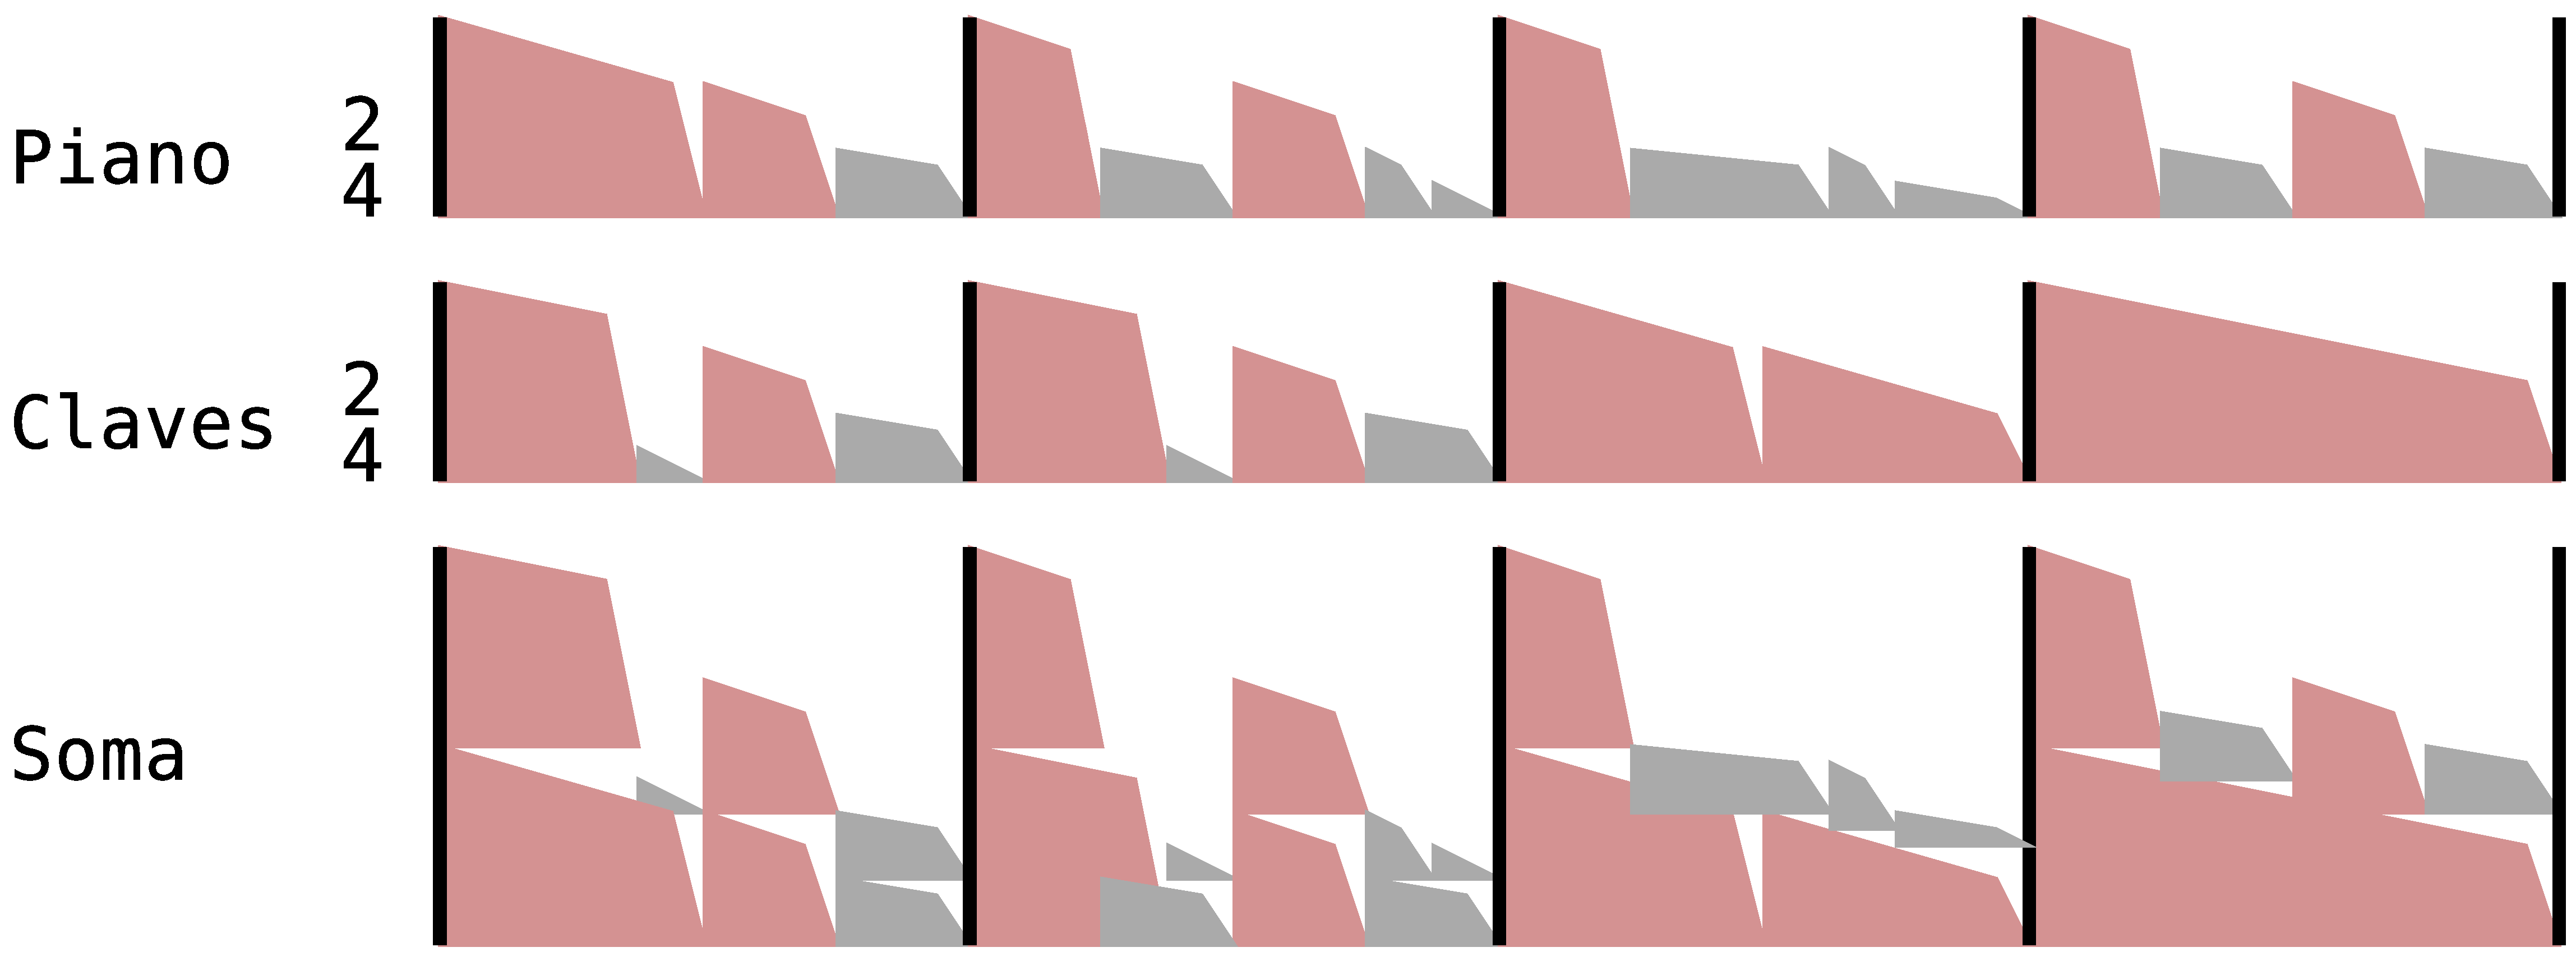
\includegraphics[width=\textwidth]{chapters/cap-musicalidade-percepcion/procurando-pulso2.eps}
\caption{Intensidades na melodia e percussão.}
\label{ritmo:procurando-pulso2}
\end{figure}
Onde temos uma aproximação do diagrama de intensidades: do piano, da clave e da soma de ambos;
no diagrama da ``soma'' fica mais claro porquê inconscientemente detetamos o fluxo de acentos,
e poderíamos inferir que este fluxo ficaria mais próximo ao fluxo do pulso, 
quando aumente o número de instrumentos envolvidos.


%%%%%%%%%%%%%%%%%%%%%%%%%%%%%%%%%%%%%%%%%%%%%%%%%%%%%%%%%%%%%%%%%%%%%%%%%%%%%%%%
\subsection{Reconhecer o tempo forte}
\index{Musicalidade!Tempo forte}
\index{Musicalidade!Bússola}
\label{subsec:perceberTF1}

\begin{wrapfigure}{r}{0.2\textwidth}
  \vspace{-10pt}
  \centering
    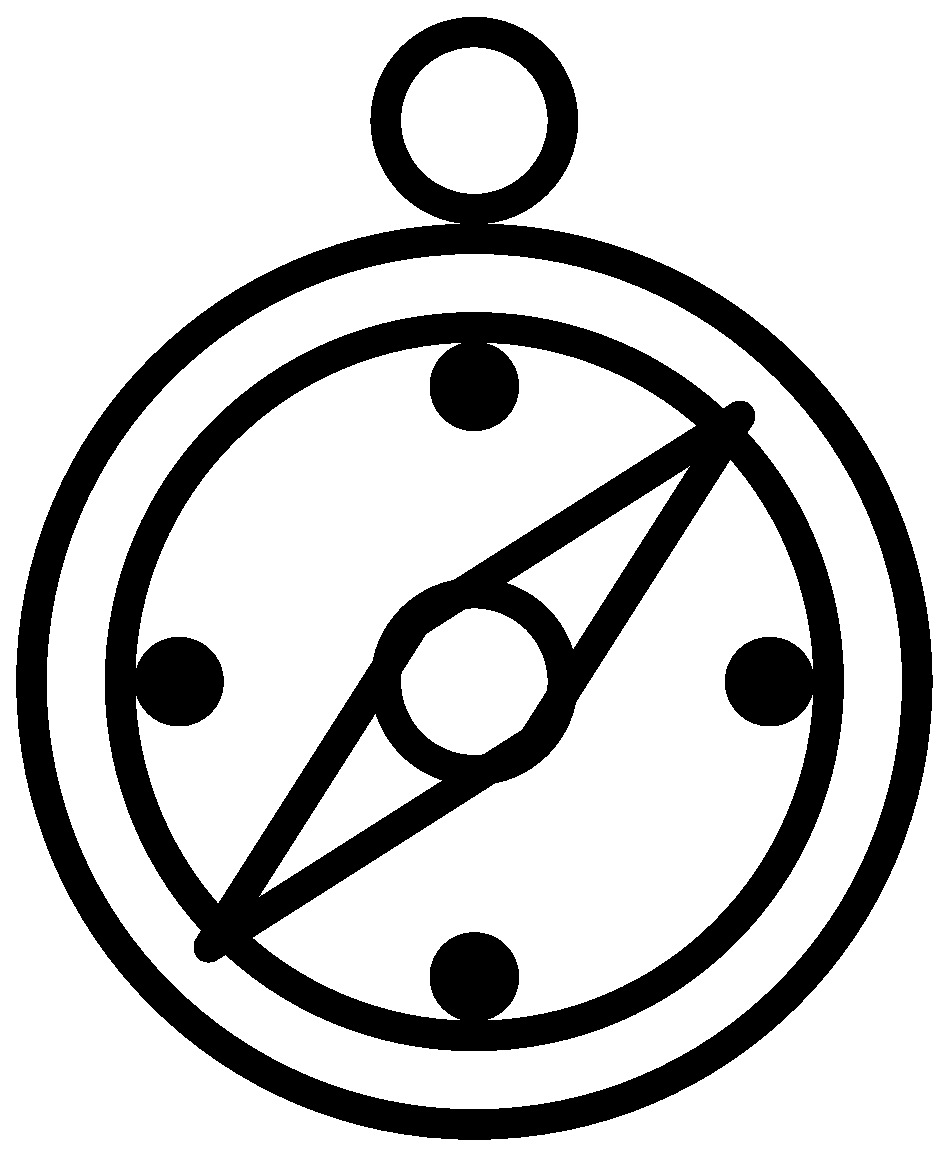
\includegraphics[width=0.15\textwidth]{compass.eps}
  \vspace{-10pt}
\end{wrapfigure}
O tempo forte é o primeiro tempo de cada \hyperref[def:Compasso]{\textbf{compasso}},
este nos ajudará a orientar-nos (bússola) em referencia à métrica da música, 
se precisamos identificá-lo numa música, podemos usar as seguintes informações:
\begin{itemize}
\item O tempo forte é o tempo em que estatisticamente percebemos que as vozes e 
instrumentos convergem executando as notas musicais com maior  \hyperref[sec:pos:Intensidade]{\textbf{intensidade}}  (potencia sonora). 
\end{itemize}

\begin{itemize}
\item Os compositores, seguindo a \hyperref[sec:ProsodiaMusical]{\textbf{prosódia musical}} vista Seção \ref{sec:ProsodiaMusical}, 
geralmente colocam as sílabas tônicas, das palavras, no tempo forte da música  \cite[pp. 149]{medteoria}. 
Da mesma forma, se fazemos um esforço de imaginação e pensamos que os instrumentos ``falam'' ou ``cantam chorando'',
podemos perceber o tempo forte identificando quê ``sílabas'' tem maior intensidade.
\item Se numa música pertencente a alguns dos \hyperref[sec:FamiliaSamba]{\textbf{subgeneros do samba}}, 
conseguimos identificar audivelmente  um padrão de repetição com a onomatopeia ``tchic-tchic tum'', 
então o tum é executado no tempo forte. 
Para mais detalhes ir a Seção \ref{sec:percepcaosamba1}.
\end{itemize}~

Lembremos que esta será uma procura do tempo forte por uma aproximação estatística, 
pois os acentos na música além de estar no tempo forte, 
também aparecem em tempos fracos, nos \hyperref[sec:contratempo]{\textbf{contratempos}}.




Além das indicações anteriores, 
existem outros critérios um pouco mais elaborados para conseguir identificar o tempo forte:
\begin{itemize}
\item Se percebemos um breque (break) na música, 
provocado por uma \hyperref[sec:Frase]{\textbf{frase}} com \hyperref[subsec:FinalAbertoFechado]{\textbf{final fechado}} 
(satisfatório, com uma sensação de ponto final), então este aconteceu no tempo forte.
\item A frase rítmica, das vozes que geram o acompanhamento da melodia principal,
geralmente iniciam no tempo forte; 
o inicio da frase é percebido com uma nota em tempo forte com maior intensidade, 
que a percebida em um tempo forte qualquer\footnote{Pode ser
devido a que se imprime de fato maior intensidade o a que mais instrumentos convergem nesse instante.}.
\end{itemize}

\begin{tcbattention}
É importante ressaltar que na música, 
a melodia principal acentua regularmente seguindo a \hyperref[def:acentometrico]{\textbf{métrica}}
e enfeita acentuando esporadicamente em \hyperref[sec:contratempo]{\textbf{contratempo}}.
Já o acompanhamento percussivo ou harmônico, por sua caraterística regular no padrão do seu ritmo,
geralmente opta por tocar continuamente acentuando no tempo forte,
ou continuamente no contratempo; 
por exemplo na música do reggae o acompanhamento geralmente está a contratempo.
\begin{itemize}
\item ``No Woman No Cry'' de Bob Marley.
\end{itemize}
\end{tcbattention}



%%%%%%%%%%%%%%%%%%%%%%%%%%%%%%%%%%%%%%%%%%%%%%%%%%%%%%%%%%%%%%%%%%%%%%%%%%%%%%%%
\subsection{Reconhecer o tipo de compasso}
\index{Musicalidade!Percepção do tipo de compasso}
\label{subsec:pertipodecompasso}
Se já conseguimos \hyperref[subsec:perceberTF1]{\textbf{identificar o tempo forte}} na música,
então podemos dizer que conhecemos o ciclo de repetição imposto pela métrica,
e podemos predizer quando acontecerá o próximo tempo forte.
Tendo em conta tudo o anterior,
o seguinte passo é deduzir quantos tempos fracos acontecem 
entre um par consecutivo de tempos fortes;
é dizer, 
temos que identificar se a música tem compassos 
\hyperref[subsec:compassobinario]{\textbf{binários}} (2 tempos), 
\hyperref[subsec:compassoternario]{\textbf{ternários}} (3 tempos), 
\hyperref[subsec:compassoquaternario]{\textbf{quaternários}} (4 tempos) 
ou outros. 

Uma forma de deduzir o tipo de compasso utilizado na música  é usando como guia o estilo musical; por exemplo:
\begin{itemize}
\item As músicas dos \hyperref[sec:FamiliaSamba]{\textbf{subgêneros do samba}} 
são principalmente escritas em compassos binários,
porém também é possível ver o uso de compassos quaternários ou de compassos compostos.
\item As músicas de forró comumente usam compassos quaternários,
porém também é possível ver o uso de compassos binários, como no baião. 
\item Em músicas usadas para dançar bolero, salsa, zouk 
e sertanejo universitário é comum perceber o uso de compassos quaternários.
\item Nas músicas onde se dança valsa são usados compassos ternários.
\item etc.
\end{itemize}
Em geral a maioria da música popular ``de moda'', no \AnoLivro, usa uma quantidade par de tempos no compasso;
sendo quaternários em primeiro lugar e binários em segundo.
Pelo que se o estilo musical não é valsa (compassos ternários), 
teremos muito provavelmente um número par de tempos no compasso;
porém, é  pouco provável atualmente achar (na rádio ou em sites de música),
o destaque de músicas em ritmo de valsa.

O método que seguiremos para identificar o tipo de compasso será testar estes tipos,
um a um, ate perceber entre eles uma maior coincidência,
iniciando o teste com o tipo de compasso com mais probabilidade seguindo o estilo musical \cite[pp. 10]{wright1992social}.
Assim, testaremos primeiro os compassos (simples)
\hyperref[subsec:compassobinario]{\textbf{binários}}, 
\hyperref[subsec:compassoternario]{\textbf{ternários}}, 
\hyperref[subsec:compassoquaternario]{\textbf{quaternários}};
se for necessário testaremos alguns compassos compostos 
e em muitas raras ocasiões os compassos mistos.

Não precisamos testar a métrica com a música como um todo,
e sim podemos usar melodias ou ritmos de instrumentos isolados para testar a métrica \cite[pp. 10]{wright1992social};
por exemplo, no caso de musicas com \hyperref[subsec:homofonica]{\textbf{textura homofônica}},
geralmente pela natureza repetitiva e marcada do acompanhamento ou da percussão,
é mais fácil detetar a métrica nessas camadas da música.

\subsubsection{Testando um compasso binário}
A forma mais simples de detetar a métrica dos compassos \hyperref[subsec:compassobinario]{\textbf{binários}},
é fazendo uma troca de peso entre nossos pés (balanço),
ate encaixar o tempo forte\footnote{Para ter certeza de que detetamos o tempo forte, 
podemos usar as técnicas explicadas na Seção \ref{subsec:perceberTF1}.} 
de um lado de nosso balanço,
e perceber que a contagem binária bate com o \hyperref[ref:Pulso]{\textbf{pulso}} da música,
e com uma distribuição de acentos, \{Forte, fraco\};
nesse ponto deduziremos de quê lado do balanço está o tempo forte e o fraco.

\begin{example}[Música com compassos de 2 tempos:]
\label{ex:compassosimples3t}
A música ``Piston de Gafieira'' de Billy Blanco,
está composta por compassos binários (simples), pelo qual tem 2 tempos.
Um exercício interessante, é \hyperref[subsec:perceberTF1]{\textbf{achar o tempo forte}},
por exemplo seguindo as sílabas tônicas na letra da música,
e tentar encaixar a contagem:\{\textbf{1}, 2\}, no ciclo da métrica, acentuando cada tempo 1 (tempo forte). 
\end{example}

\begin{example}[Outros exemplos de compassos binários:]
~
\begin{itemize}
\item ``Tico-Tico no fubá'' de Zequinha de Abreu  \cite[pp. 6]{marcondes1998enciclopedia} \cite[pp. 39,91]{diniz2003almanaque}.
\item ``Brasileirinho'' de Valdir Azevedo  \cite[pp. 133]{perna2002samba}.
\item ``Pelo telefone'' de  Ernesto dos Santos (Donga) e Mauro de almeida.
\item ``Pierrô apaixonado'' de Heitor dos prazeres e Noel Rosa \cite[pp. 1070]{marcondes1977enciclopediav2} \cite[pp. 53]{diniz2008almanaque}.
\item ``A banda'' de Chico Buarque interpretada por Nara Leão \cite[pp. 90]{diniz2008almanaque} \cite{partituraabanda1}.
\end{itemize}
\end{example}


\subsubsection{Testando um compasso ternário}
Neste caso bastará que nós contemos ate 3, iniciando em 1 no tempo forte,
e procurando que os três tempos encaixem perfeito no ciclo da métrica (entre dois tempos fortes consecutivos).
Se percebemos que esta contagem encaixa na métrica,
com uma distribuição de acentos, \{Forte, fraco, fraco\} \cite[pp. 10]{wright1992social}, 
então estamos sim, frente a um  \hyperref[subsec:compassoternario]{\textbf{compasso ternário}}.

\begin{example}[Música com compassos de 3 tempos:]
\label{ex:compassosimples3t3}
A música ``João e Maria'' de Chico Buarque,
está composta por compassos ternários (simples), pelo qual tem 3 tempos.
Um exercício interessante, é \hyperref[subsec:perceberTF1]{\textbf{achar o tempo forte}},
por exemplo seguindo as sílabas tônicas na letra da música,
e tentar encaixar a sequencia:\{\textbf{1}, 2 , 3\}, no ciclo da métrica,acentuando cada tempo 1 (tempo forte). 
\end{example}

\begin{example}[Outros exemplos de compassos ternários:]
\label{ex:compassosimples3t2}
~
\begin{itemize}
\item ``Rio grande tchê'' interpretado pelo grupo Os serranos.
\item ``Blusa Vermelha'' interpretado pelo Trio Parada Dura.
%\item ``Ainda ontem chorei de saudade'' interpretado por Eduardo Costa e Leonardo.
\item ``Último adeus'' interpretado por Eduardo Costa e Leonardo.
\item ``Chao de Giz'' de Ze Ramalho.
\end{itemize}
\end{example}

\subsubsection{Testando um compasso quaternário}
Neste caso nos temos que contar ate 4, iniciando em 1 no tempo forte,
e procurando que os quatro tempos encaixem perfeito no ciclo da métrica.
Se percebemos que esta contagem encaixa na métrica (entre dois tempos fortes consecutivos),
com uma distribuição de acentos, \{Forte, fraco, meio forte, fraco\} \cite[pp. 10]{wright1992social}, 
então estamos sim, frente a um  \hyperref[subsec:compassoquaternario]{\textbf{compasso quaternário}}.


\begin{example}[Música com compassos de 4 tempos:]
\label{ex:compassosimples4t}
A música (\hyperref[subsec:marcha]{\textbf{Marcha}}) ``Noite dos Mascarados'' de Chico Buarque,
está composta por compassos quaternários (simples), pelo qual tem 4 tempos,
e podemos contar: \{\textbf{1}, 2 , 3, 4\}, acentuando cada tempo 1 (tempo forte) e cada tempo 3 (tempo semi forte).
Um exercício interessante, é \hyperref[subsec:perceberTF1]{\textbf{achar o tempo forte}},
por exemplo seguindo as sílabas tônicas na letra da música,
e tentar encaixar a sequencia da contagem no ciclo da métrica, 
\end{example}

\begin{example}[Outros exemplos de compasso quaternário:]
~
\begin{itemize}
\item ``Sambolero'' interpretado por Luiz Bonfá \cite[pp. 49]{sambolero}.
\item ``Cê que sabe'' interpretado por Cristiano Araujo.
\item ``Vai dar namoro'' interpretado por Bruno e Marrone.
\item ``Vou te amarrar a minha cama'' interpretado por Bruno e Marrone.
\item ``Borbulhas de amor'' interpretado por Eduardo costa e Leonardo%Gustavo Lima.
\end{itemize}
\end{example}

\subsubsection{Compassos compostos}
Na prática, bastará a principio, para um dançarino iniciante,
reconhecer os compassos \hyperref[subsec:compassoquaternario]{\textbf{quaternários}}, 
\hyperref[subsec:compassobinario]{\textbf{binários}}, e 
\hyperref[subsec:compassoternario]{\textbf{ternários}},
nesse ordem de ocorrência;
pois as raras ocasiões onde estejamos frente a um \hyperref[sec:compaso]{\textbf{compasso composto}},
um dançarino pode tratar ele como sua contraparte simples,
e desenvolver-se suficientemente bem na dança. 
Podemos perceber o uso de compassos compostos de 6 pulsos nos Exemplos \ref{ex:compassocomposto6}
e \ref{ex:compassocomposto6b},
este tipo de compassos é muito comum nas baladas pop e na música erudita.
\begin{example}[Música com compassos de 6 pulsos:]
\label{ex:compassocomposto6}
Um exemplo deste tipo de música pode ser escutado em ``A Thousand Years'', 
interpretado por Christina Perri. É fácil perceber como podemos nos confundir,
pensando que a música usa compassos binários (simples) de andamento lento,
ou ternários de andamento rápido; quando na realidade trata-se de compassos binários compostos de 6 pulsos (dois tempos),
possivelmente com formula de compasso 6/8.

Um dançarino, mesmo sabendo que trata-se de um \hyperref[compasso:binario]{\textbf{compasso binário composto}} (de 6 pulsos),
pode tratar a música como se esta fosse binária simples, e dançar em grupos de dois passos lentos,
ou como se fosse ternaria simples, e tentar dançar estilo valsa porém muito rápida.

A mínima subdivisão a ser feita por nós na dança, 
será a de assumir um compasso binário, usando movimentos binários,
pois quando tentemos subdividir por dois um passo, para encaixar um ``tchic tchic tum'',
acharemos a dança desconfortável, devido a que
entraremos em conflito com o \hyperref[ref:Pulso]{\textbf{pulso}}, 
que divide o compasso em porções múltiplos de três.
  
\end{example}

\begin{example}[Outros exemplos de compassos binários de 6 pulsos:]
\label{ex:compassocomposto6b}
~
\begin{itemize}
\item ``Quem é ela'' interpretado por Marco e Mário.
\item ``Seu amor ainda é tudo'' interpretado por Eduardo Costa e Leonardo.
\item ``You don't own me'' interpretado por Grace.
\item ``We are the champions'' interpretado pelo grupo Queen.
\item ``Hallelujah'' interpretado por Rufus Wainwright.
\item ``Happy Christmas'' interpretado por John Lennon.
\item ``The House of the Rising Sun'' interpretado pelo grupo  The Animals.
%\item ``Lakmé'' interpretado por Léo Délibes.
%\item ``Nothing Else Matters'' interpretado pelo grupo Metallica.
\end{itemize}
\end{example}

\subsubsection{Compassos mistos}
Em muitas raras ocasiões, mais raro ainda que o caso dos compassos compostos, 
podemos achar compassos mistos, como nos Exemplos \ref{ex:compassomisto5} e \ref{ex:compassomisto7}.

\begin{example}[Música com compassos de 5 pulsos:]
\label{ex:compassomisto5}
A música ``Take Five'' interpretada por  Dave Brubeck,
está composta por compassos mistos (alternados), criados pela concatenação de um compasso binário e um ternário,
contando-se os tempos: \{\textbf{1}, 2, \textbf{1}, 2, 3\}, acentuando o 1.
Um exercício interessante, é achar o tempo forte  e tentar encaixar esta sequencia na música, 
\end{example}

\begin{example}[Música com compassos de 7 pulsos:]
\label{ex:compassomisto7}
A música ``Money'' interpretada pela banda  Pink Floyd,
esta composta por compassos mistos (alternados), criados pela concatenação de um compasso quaternário e um ternário,
contando-se os tempos: \{\textbf{1}, 2 , 3, 4, \textbf{1}, 2, 3\}, acentuando cada tempo 1 e o primeiro 3 (meio forte).
Um exercício interessante, é achar o tempo forte  e tentar encaixar esta sequencia na música, 
\end{example}

%%%%%%%%%%%%%%%%%%%%%%%%%%%%%%%%%%%%%%%%%%%%%%%%%%%%%%%%%%%%%%%%%%%%%%%%%%%%%%%%
%%%%%%%%%%%%%%%%%%%%%%%%%%%%%%%%%%%%%%%%%%%%%%%%%%%%%%%%%%%%%%%%%%%%%%%%%%%%%%%%
\section{Percepção da métrica no samba}
\index{Musicalidade!Métrica no samba}
\label{sec:percepcaosamba1}

As músicas dos subgêneros do samba, que usamos para dançar, 
geralmente são escritas usando \hyperref[subsec:compassobinario]{\textbf{compassos binários}};
pelo que, a procura da métrica das musicas destes subgêneros,
é mais simples, 
pois iniciamos a busca tendo a quase certeza do tipo do compasso, 
só precisaríamos \hyperref[subsec:perceberTF1]{\textbf{achar o tempo forte}} 
usando as indicações descritas na seção \ref{subsec:perceberTF1}.

Assim, para detetar o tempo forte e as \hyperref[sec:pos:Duracion]{\textbf{durações}} dos tempos nos compassos,
devemos ter em conta que quando escutamos uma música, 
na qual é tipicamente dançado o samba, ou especificamente o samba de gafieira,
podemos distinguir que a soma dos sons produzidos pelos instrumentos de percussão\footnote{Ou o
acompanhamento em geral.}, 
geram um padrão de repetição muito particular, 
geralmente relacionado com as onomatopeias: ``tchic tchic tum'' ou ``tum tum'';
onde em ambos  casos existe um  ``tum'' executado com maior 
\hyperref[sec:pos:Intensidade]{\textbf{intensidade}} (potencia sonora),
que está sendo executado-se no tempo forte.
Se conseguimos detetar alguma das duas onomatopeias,
então temos o problema resolvido, pois ambas ocupam exatamente dois tempos,
e dado que para conseguir encaixar as onomatopeias tivemos que reconhecer o tempo forte no ``tum'',
temos todos os elementos para descrever a métrica no tempo da música.

\PRLsep{Analisando a música no samba}

A Figura \ref{fig:abc-caquarela} representa os compassos 18, 19 e 20 da  
composição musical ``Aquarela do Brasil'' escrita
por Ary Barroso em 1939 \cite{AquarelaDoBrasil}; 
a versão mostrada na figura teve arranjos por Irineu Krüger \cite{Irineu}. 
\begin{figure}[ht]
\centering
%\includegraphics[width=\textwidth]{chapters/cap-fundamentos/aquarela.png}
\begin{abc}[name=abc-caquarela]%,options={-O= -c -s 0.8}]
% abcm2ps aquarela.abc  -O aquarela.ps
% ps2epsi aquarela.ps aquarela.eps
%
X: 1 % start of header
T: Brazil - Aquarela do Brasil
C: Music: Ary Barroso, 1939
C: Arranged by: Irineu Krüger
K: C % scale: C major
M: 2/4 % formula do compasso
%
V:1 clef=treble name="Voice Choir" sname="Voice Choir"
V:2 clef=treble name="Eb" sname="Eb"
V:3 clef=treble name="Bb" sname="Bb"
V:4 clef=treble name="Strings" sname="Strings"
V:5 clef=bass   name="D. Bass" sname=""D. Bass"
%
%
[V:1] "18" C'3/2A/2C2  |"19" A3/2(G/2 G/2)E1E/2  |"20" z/2 C'1A/2 C'1C'1  |
w:    Ó Bras-sil        sam-ba_ que dá       bam-bo-leio_ 
w:    Ó Bras-sil        ver-de que dá_       pa-ra~o mun-do 
%
%
[V:2] G1z/2G1z/2G1  | G1z/2G1z/2G1  | G1z/2G1z/2G1  |
%
%
[V:3] z4  | z4  | z4  |
%
%
[V:4] G1z/2G1z/2G1  | G1z/2G1z/2G1  | G1z/2G1z/2G1  |
%
%
[V:5] C,2 G,,2  | C,1 z1 G,,2  | C,2 G,,2  |
\end{abc}
\caption{3 compassos da partitura da composição ``Aquarela do brasil''}
\label{fig:abc-caquarela}
\end{figure}
Nesta versão, a música está escrita seguindo uma 
\hyperref[subsec:homofonica]{\textbf{textura homofônica}} com:
\begin{itemize}
\item \textbf{melodia principal:} 1 voz ou coro de voces (``Voice Choir'') e  
\item \textbf{acompanhamento:} 4 instrumentos (``Eb'',``Bb'',``Strings'' e ``D. Bass''), 
\end{itemize}
que usam uma 
formula de compasso $2/4$, de modo que se tem compassos
binários com tempos com uma \hyperref[sec:pos:Duracion]{\textbf{duração}} de uma semínima (\quarternote).

\subsection{Percepção do: tchic-tchic tum}
Analisando o fragmento de partitura da Figura \ref{fig:abc-caquarela} e escutando a música produzida, 
podemos perceber que os instrumentos executados em conjunto geram um sonido identificável
com a onomatopeia ``tchic tchic tum'', com uma duração de dois tempos.
Assim, o inicio de cada compasso coincide com o ``tum''; 
sendo que este é o momento em que a maioria dos instrumentos produzem um sonido, 
de modo que a sensação para o ouvinte é de uma potencia sonora maior. 
Cada instrumento prolongará seu sonido de forma diferente; 
porem,  podemos dizer que: o ``tum'' ocupa $1$ tempo (\quarternote), 
e que o sonido de um ``tchic'' ocupa médio tempo (0.5\quarternote),
sendo que o primeiro ``tchic'' é executado no tempo fraco de ``D. Bass'', 
e o segundo ``tchic'' solapa e obscurece ao  primeiro, 
que é executado na parte fraca do tempo fraco de ``Strings'' ou ``Eb'' (fazendo um \hyperref[sec:contratempo]{\textbf{contratempo}});
conseguindo assim criar a ilusão da onomatopeia ``tchic tchic tum'', 
com ``tchic''s de médio tempo; de modo que:
\begin{equation}
tchic + tchic = tum ~~ \Longleftrightarrow ~~ tchic = \frac{tum}{2}.
\end{equation}
 
Por outro lado, se a percepção do ouvinte é mais
aguçada, poderá escutar a onomatopeia: ``a tchic-tchic tum''; 
neste caso, o sonido ``tum'' é solapado por o sonido de ``a'',
quando transcorrido um $75\%$ do primeiro tempo do compasso; 
o sonido ``a''  se prolonga incluindo a parte forte do tempo fraco subsequente, 
este sonido é executado pelos instrumentos ``Eb'' e ``Strings'' e constitui uma 
\hyperref[sec:sincope]{\textbf{sincope}} \cite[pp. 143]{medteoria}.


Pelo exposto anteriormente, 
podemos simplificar o acompanhamento na partitura para gerar um sonido com onomatopeia
``tchic tchic tum'', como o mostrado na Figura \ref{fig:abc-contratempo1}.
\begin{figure}[ht]
\centering
\begin{abc}[name=abc-contratempo1,width=0.75\linewidth]
X: 1 % start of header
K: C % scale: C major
M:2/4
%T: Contratempo num compasso binário
V:1 clef=treble name="Instrumento 1" sname="Inst. 1"
V:2 clef=bass   name="Instrumento 2" sname="Inst. 2"
[V:1] |: " ""T/2"G1 " ""T/2"z1 " ""T/2"z1 " ""T/2"G1 | " ""T/2"G1 " ""T/2"z1 " ""T/2"z1 " ""T/2"G1  :|
w:    tum                tchic                       tum                   tchic           
[V:2] |:  "Tempo"C,2 "Tempo"G,,2  | "Tempo"C,2 "Tempo"G,,2  :|
w:    tum       tchic              tum       tchic            
\end{abc}
\caption{Padrão de repetição para gerar um sonido de onomatopeia ``tchic tchic tum''.}
\label{fig:abc-contratempo1}
\end{figure}
Onde o instrumento 1 executa dois sonidos, de modo que o primeiro contribui ao sonido 
``tum'' e o segundo sonido gera o segundo ``tchic'' do compasso; por outro lado,
o instrumento 2 executa um ritmo com um padrão
de repetição de dois sonidos ``tum'' e ``tchic'', nesse ordem;
sendo que a nota executada no tempo forte produz um sonido mais agudo que a 
executada no tempo fraco, isto é assim para poder diferenciar melhor ambos tempos.

\begin{figure}[!h]
\begin{elaboracion}[title=Samba: Ritmo vs. Fala]
\index{Música!Ritmo vs. Fala}
Quando reconhecemos o ritmo do samba com a onomatopeia ``tchic tchic tum'', 
podemos perceber que existe uma contradição, entre 
o que percebemos ao escutar uma música, e a forma como esta é realmente escrita nos compassos na partitura.
Pois como é visto na Figura \ref{fig:abc-contratempo1}, quando escrevemos
um ritmo com um padrão de repetição na ordem ``tum tchic tchic'', 
para o ouvinte é mais natural associar e pensar
que se está executando um ritmo com um padrão ``tchic tchic tum'', 
devido a que quando um ser humano fala, este usa a pausa
para denotar o final de uma palavra. Assim, ao escutar o padrão ``tum tchic tchic'', 
nossa mente otimizada para detetar palavras,
associa que o sonido que tem um silencio maior apos ser executado,
neste caso o ``tum'', marca o final do ciclo do padrão de repetição (a palavra). 

Pelo que quando um músico vê, ao ler uma partitura, 
um padrão de repetição ``tum tchic tchic''; 
um ouvinte interpretará de forma instintiva que o padrão é ``tchic tchic tum'' iniciando em ``tchic''.
Porem não devemos confundir-nos, o ``tum'' é executado no tempo 1 do compasso.
\end{elaboracion}
\label{fig:RitmoVsFala}
\end{figure}

\subsection{Percepção do: tum~tum}

Analisando o fragmento de partitura, da Figura \ref{fig:abc-caquarela}, 
e tentando escutar os compassos, 
para audivelmente isolar o instrumento ``D. Bass'' (que é o bumbo),
podemos perceber que este gera um sonido, 
com um \hyperref[sec:pos:Altura]{\textbf{tom}} muito grave, 
identificável com a onomatopeia ``tum tum'', com uma duração de dois tempos.
No samba este ritmo é muito identificável na maioria das musicas,
e pode servi-nos de referencia à hora de dançar ou simplesmente tentar achar o pulso.
Este instrumento é descrito isoladamente na Figura \ref{fig:abc-contratempo1tumtum},
onde podemos apreciar que o compositor achou interessante diferenciar o tom,
 do som que gerava o bumbo, em cada tempo;
neste caso, um som mais agudo para o tempo forte e um mais grave para o tempo fraco;
porem esta diferença não é uma regra, pelo que se estamos procurando achar os tempos da música escutando o bumbo,
o melhor é simplesmente tentar perceber qual está sendo tocado com maior \hyperref[sec:pos:Intensidade]{\textbf{intensidade}}.
\begin{figure}[ht]
\centering
\begin{abc}[name=abc-contratempo1tumtum,width=0.75\linewidth]
X: 1 % start of header
K: C % scale: C major
M:2/4
%T: Contratempo num compasso binário
V:1 clef=bass   name="D. Bass" sname="D. Bass"      
[V:1] |: "Tempo"C,2 "Tempo"G,,2  | "Tempo"C,2 "Tempo"G,,2  :|
w:    tum       tum         tum       tum            
\end{abc}
\caption{Padrão de repetição para gerar um sonido de onomatopeia ``tum tum''.}
\label{fig:abc-contratempo1tumtum}
\end{figure}


%%%%%%%%%%%%%%%%%%%%%%%%%%%%%%%%%%%%%%%%%%%%%%%%%%%%%%%%%%%%%%%%%%%%%%%%%%%%%%%%
%%%%%%%%%%%%%%%%%%%%%%%%%%%%%%%%%%%%%%%%%%%%%%%%%%%%%%%%%%%%%%%%%%%%%%%%%%%%%%%%
\section{Percepção rítmica (exercícios)}
\index{Musicalidade!Percepção rítmica}



Como já foi visto na Seção \ref{sec:percepcaosamba1},
existem um conjunto de onomatopeias, que representam  tradicionalmente,
aos ritmos  que acompanham à melodia principal, 
nas músicas que pertencem aos \hyperref[sec:FamiliaSamba]{\textbf{subgêneros do samba}};
estes ritmos de acompanhamento, ou as simplificações que percebemos, 
geralmente tem um padrão muito homogêneo entre compassos sucessivos,
de modo que são muito fáceis de predizer para um dançarino, 
e estes podem servir de guia ou como um porto seguro.

Assim, esses ritmos simples, geralmente são usados como uma forma que emoldura a execução dos passos básicos,
e alguns mais complexos;
porem, existem passos ou movimentos no samba de gafieira e outros estilos de dança,
que se saem desses padrões rítmicos simples. 
\begin{itemize}
\item Em alguns casos,
isto é feito para agregar artisticamente um pouco de complexidade aos movimentos,
porem sem sair-nos completamente da guia do ritmo do acompanhamento; mas 
\item em outros casos, nos saímos dos padrões desse ritmo, 
porque deixamos de seguir o ritmo do acompanhamento,
e iniciamos a seguir o ritmo da melodia principal, que geralmente é mais complexa,
e muito heterogênea entre compassos sucessivos\footnote{Este 
tema será abordado mais amplamente na Seção \ref{sec:aspectosusicalidade}.}. 
\end{itemize}


Nesta seção serão presentadas uma serie dinâmicas grupais, 
para decorar e acostuma-nos ao uso dos ritmos mais simples e comuns, 
a serem usados no acompanhamento do samba de gafieira e outros estilos de dança.

Nestos exemplos, está escrito com maiúscula a onomatopeia 
que cai no tempo com acento métrico, para lembrar este detalhe na execução do som. 
Também, além de uma pauta para descrever os exemplos, 
é desenhada uma representação num diagrama circular,
para facilitar a leitura e execução da pauta.
Nesse diagrama, os círculos pretos representam notas executadas em tempo forte,
e os círculos cinza, as notas executadas num tempo fraco;
a leitura do diagrama deve ser feito em sentido horário.  

\begin{example}[Treinamentos simples:]
Um professor, ou um software programado, 
deve executar, uma ou duas vesses, alguma das sequencias rítmicas mostradas nas Figuras 
\ref{fig:abc-percepcionritmica1}, \ref{fig:abc-percepcionritmica2},
\ref{fig:abc-percepcionritmica3}  e \ref{fig:abc-percepcionritmica4}.
Seguidamente os estudantes devem lembrar e repetir o ritmo, 
incluindo as acentuações, dando palmas ou batendo com os pés.
\end{example}


\begin{figure}[H]
\centering
     \begin{subfigure}[c]{0.45\textwidth}
         \centering
         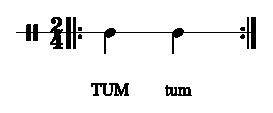
\includegraphics[width=\textwidth]{chapters/cap-musicalidade-percepcion/treino-ritmo1-1.eps}
         \caption{Pauta do ritmo.}
         \label{fig:RitmoTUMtum1}
     \end{subfigure}
     \hfill
     \begin{subfigure}[c]{0.45\textwidth}
         \centering
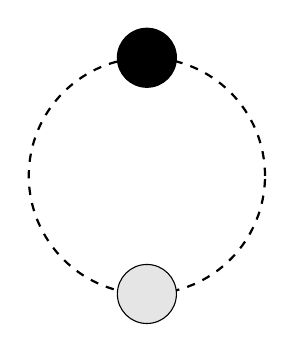
\begin{tikzpicture}
\pgfmathsetmacro{\RadioTot}{1.5}
\pgfmathsetmacro{\Base}{4}
\pgfmathsetmacro{\Radio}{\RadioTot/\Base}
\pgfmathsetmacro{\Theta}{360/\Base}

\draw[black,thick,dashed] (0,0) circle (\RadioTot cm);

\foreach \x in {2}
{
	\draw  [black,fill=gray!20] ({\RadioTot*cos(90-\x*\Theta )} ,{\RadioTot*sin(90-\x*\Theta )})circle (\Radio cm);
}

\foreach \x in {0}
{
	\draw  [black,fill=black] ({\RadioTot*cos(90-\x*\Theta )} ,{\RadioTot*sin(90-\x*\Theta )})circle (\Radio cm);
}
\end{tikzpicture}
         \caption{Diagrama circular do ritmo.}
         \label{fig:RitmoTUMtum2}
     \end{subfigure}
\caption{Descrição do ritmo.}
\label{fig:abc-percepcionritmica1}
\end{figure}


\begin{figure}[H]
\centering
     \begin{subfigure}[c]{0.45\textwidth}
         \centering
         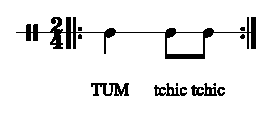
\includegraphics[width=\textwidth]{chapters/cap-musicalidade-percepcion/treino-ritmo2-1.eps}
         \caption{Pauta do ritmo.}
         \label{fig:RitmoTUMtchictchic1}
     \end{subfigure}
     \hfill
     \begin{subfigure}[c]{0.45\textwidth}
         \centering
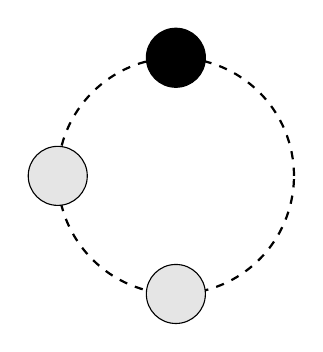
\begin{tikzpicture}
\pgfmathsetmacro{\RadioTot}{1.5}
\pgfmathsetmacro{\Base}{4}
\pgfmathsetmacro{\Radio}{\RadioTot/\Base}
\pgfmathsetmacro{\Theta}{360/\Base}

\draw[black,thick,dashed] (0,0) circle (\RadioTot cm);

\foreach \x in {2,3}
{
	\draw  [black,fill=gray!20] ({\RadioTot*cos(90-\x*\Theta )} ,{\RadioTot*sin(90-\x*\Theta )})circle (\Radio cm);
}

\foreach \x in {0}
{
	\draw  [black,fill=black] ({\RadioTot*cos(90-\x*\Theta )} ,{\RadioTot*sin(90-\x*\Theta )})circle (\Radio cm);
}
\end{tikzpicture}
         \caption{Diagrama circular do ritmo.}
         \label{fig:RitmoTUMtchictchic2}
     \end{subfigure}
\caption{Descrição do ritmo.}
\label{fig:abc-percepcionritmica2}
\end{figure}

\begin{figure}[H]
\centering
     \begin{subfigure}[c]{0.45\textwidth}
         \centering
         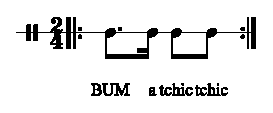
\includegraphics[width=\textwidth]{chapters/cap-musicalidade-percepcion/treino-ritmo3-1.eps}
         \caption{Pauta do ritmo; $BUM=\frac{3}{4}TUM$.}
         \label{fig:RitmoTUMatchictchic1}
     \end{subfigure}
     \hfill
     \begin{subfigure}[c]{0.45\textwidth}
         \centering
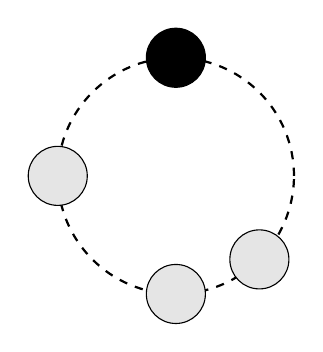
\begin{tikzpicture}
\pgfmathsetmacro{\RadioTot}{1.5}
\pgfmathsetmacro{\Base}{4}
\pgfmathsetmacro{\Radio}{\RadioTot/\Base}
\pgfmathsetmacro{\Theta}{360/\Base}

\draw[black,thick,dashed] (0,0) circle (\RadioTot cm);

\foreach \x in {1.5,2,3}
{
	\draw  [black,fill=gray!20] ({\RadioTot*cos(90-\x*\Theta )} ,{\RadioTot*sin(90-\x*\Theta )})circle (\Radio cm);
}

\foreach \x in {0}
{
	\draw  [black,fill=black] ({\RadioTot*cos(90-\x*\Theta )} ,{\RadioTot*sin(90-\x*\Theta )})circle (\Radio cm);
}
\end{tikzpicture}
         \caption{Diagrama circular do ritmo.}
         \label{fig:RitmoTUMatchictchic2}
     \end{subfigure}
\caption{Descrição do ritmo.}
\label{fig:abc-percepcionritmica3}
\end{figure}


\begin{figure}[H]
\centering
     \begin{subfigure}[c]{0.45\textwidth}
         \centering
         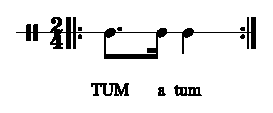
\includegraphics[width=\textwidth]{chapters/cap-musicalidade-percepcion/treino-ritmo4-1.eps}
         \caption{Pauta do ritmo; $BUM=\frac{3}{4}TUM$}
         \label{fig:RitmoTUMatum1}
     \end{subfigure}
     \hfill
     \begin{subfigure}[c]{0.45\textwidth}
         \centering
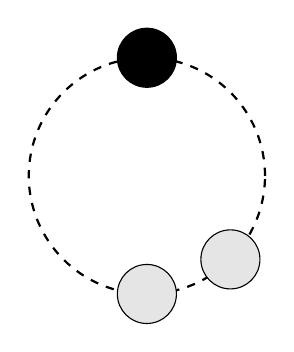
\begin{tikzpicture}
\pgfmathsetmacro{\RadioTot}{1.5}
\pgfmathsetmacro{\Base}{4}
\pgfmathsetmacro{\Radio}{\RadioTot/\Base}
\pgfmathsetmacro{\Theta}{360/\Base}

\draw[black,thick,dashed] (0,0) circle (\RadioTot cm);

\foreach \x in {1.5,2}
{
	\draw  [black,fill=gray!20] ({\RadioTot*cos(90-\x*\Theta )} ,{\RadioTot*sin(90-\x*\Theta )})circle (\Radio cm);
}

\foreach \x in {0}
{
	\draw  [black,fill=black] ({\RadioTot*cos(90-\x*\Theta )} ,{\RadioTot*sin(90-\x*\Theta )})circle (\Radio cm);
}
\end{tikzpicture}
         \caption{Diagrama circular do ritmo.}
         \label{fig:RitmoTUMatum2}
     \end{subfigure}
\caption{Descrição do ritmo.}
\label{fig:abc-percepcionritmica4}
\end{figure}

\begin{example}[Treinamentos elaborados:]
Um professor, ou um software programado, 
deve executar muitas vesses, por exemplo 32, 
as sequencias rítmicas mostradas nas Figuras 
\ref{fig:abc-percepcionritmica5} e \ref{fig:abc-percepcionritmica6}.
Enquanto que os estudantes acompanham o ritmo, 
incluindo as acentuações, dando palmas ou batendo com os pés\footnote{Pode
ser divertido indicar que se pode andar e criar movimentos com os pés, 
sempre que se respeite o ritmo proposto.},
de jeito que a sincronia seja perfeita.
\end{example}

\begin{figure}[H]
\centering
     \begin{subfigure}[c]{0.45\textwidth}
         \centering
         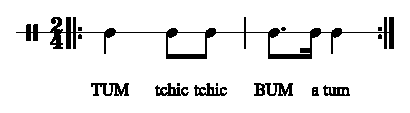
\includegraphics[width=\textwidth]{chapters/cap-musicalidade-percepcion/treino-ritmo5-1.eps}
         \caption{Pauta do ritmo; $BUM=\frac{3}{4}TUM$}
         \label{fig:Ritmocomplexo1:1}
     \end{subfigure}
     \hfill
     \begin{subfigure}[c]{0.45\textwidth}
         \centering
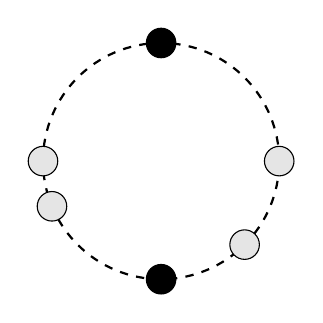
\begin{tikzpicture}
\pgfmathsetmacro{\RadioTot}{1.5}
\pgfmathsetmacro{\Base}{8}
\pgfmathsetmacro{\Radio}{\RadioTot/\Base}
\pgfmathsetmacro{\Theta}{360/\Base}

\draw[black,thick,dashed] (0,0) circle (\RadioTot cm);

\foreach \x in {2,3,5.5,6}
{
	\draw  [black,fill=gray!20] ({\RadioTot*cos(90-\x*\Theta )} ,{\RadioTot*sin(90-\x*\Theta )})circle (\Radio cm);
}

\foreach \x in {0,4}
{
	\draw  [black,fill=black] ({\RadioTot*cos(90-\x*\Theta )} ,{\RadioTot*sin(90-\x*\Theta )})circle (\Radio cm);
}
\end{tikzpicture}
         \caption{Diagrama circular do ritmo.}
         \label{fig:Ritmocomplexo1:2}
     \end{subfigure}
\caption{Descrição do ritmo.}
\label{fig:abc-percepcionritmica5}
\end{figure}





\begin{figure}[H]
\centering
     \begin{subfigure}[c]{0.45\textwidth}
         \centering
         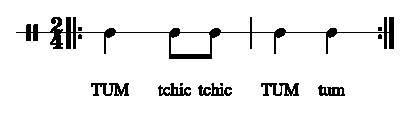
\includegraphics[width=\textwidth]{chapters/cap-musicalidade-percepcion/treino-ritmo6-1.eps}
         \caption{Pauta do ritmo.}
         \label{fig:Ritmocomplexo2:1}
     \end{subfigure}
     \hfill
     \begin{subfigure}[c]{0.45\textwidth}
         \centering
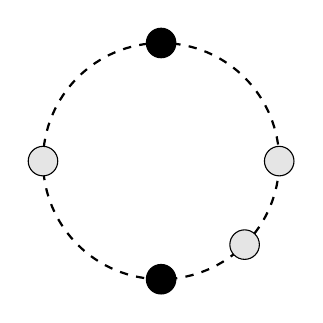
\begin{tikzpicture}
\pgfmathsetmacro{\RadioTot}{1.5}
\pgfmathsetmacro{\Base}{8}
\pgfmathsetmacro{\Radio}{\RadioTot/\Base}
\pgfmathsetmacro{\Theta}{360/\Base}

\draw[black,thick,dashed] (0,0) circle (\RadioTot cm);

\foreach \x in {2,3,6}
{
	\draw  [black,fill=gray!20] ({\RadioTot*cos(90-\x*\Theta )} ,{\RadioTot*sin(90-\x*\Theta )})circle (\Radio cm);
}

\foreach \x in {0,4}
{
	\draw  [black,fill=black] ({\RadioTot*cos(90-\x*\Theta )} ,{\RadioTot*sin(90-\x*\Theta )})circle (\Radio cm);
}
\end{tikzpicture}
         \caption{Diagrama circular do ritmo.}
         \label{fig:Ritmocomplexo2:2}
     \end{subfigure}
\caption{Descrição do ritmo.}
\label{fig:abc-percepcionritmica6}
\end{figure}

\newpage
%%%%%%%%%%%%%%%%%%%%%%%%%%%%%%%%%%%%%%%%%%%%%%%%%%%%%%%%%%%%%%%%%%%%%%%%%%%%%%%%
%%%%%%%%%%%%%%%%%%%%%%%%%%%%%%%%%%%%%%%%%%%%%%%%%%%%%%%%%%%%%%%%%%%%%%%%%%%%%%%%
\section{Percepção de frases musicais}
\label{sec:perceberfrases}
\index{Musicalidade!Frase musical}

Como foi visto na Seção \ref{sec:Frase}, 
as \hyperref[sec:Frase]{\textbf{frases musicais}} podem ser classificadas seguindo seu tipo de inicio e final. 
A composição estruturada que envolve os critérios que são usados para agrupar frases musicais em estruturas maiores 
é estudada nas seções \ref{sec:fraseio}, \ref{sec:estruturadamusica} e \ref{sec:compondoestruturadamente}. 
Um par de exemplos simples destas estruturas formadas por frases 
foram vistos quando estudamos os \hyperref[sec:Periodo]{\textbf{períodos}} e 
as \hyperref[sec:sentence]{\textbf{sentenças}} nas Seções \ref{sec:Periodo} e \ref{sec:sentence}, 
respetivamente.

Nesta seção presentaremos critérios para poder dividir uma música ou uma seção dela 
nas suas frases musicais. 


\begin{tcbattention}
Uma coisa importante a ter em conta quando analisamos as frases numa música 
é que estas tendem a ser percebidas de forma irregular na introdução da música;
porque nessa seção da peça os compositores tem muita liberdade criativa
e costumam introduzir irregularidades no comprimento da frase em relação ao corpo da peça. 
Por isso é recomendável iniciar nosso analises das frases no corpo da música. 
\end{tcbattention}

\subsection{Separando frases analiticamente}

Para poder identificar as frases musicais,
nesta seção serão presentadas algumas dicas extraídas da teoria musical,
pelo que seu uso requer um mínimo de conhecimento teórico nesta área. 



\PRLsep{Frases de comprimento regular}

Na música popular, podemos achar peças com frases musicais com um comprimento regular,
ou seja que  tem a mesma quantidade de compassos em toda a música;
nesse caso, uma forma de identificar e separar as frases musicais  
é detetando uma frase na peça musical,
contar o número de compassos que esta contem  
e usar esta medida para detetar e predizer as demais frases.


\begin{itemize}
\item Os comprimento de frase de 4 e 8 compassos 
são os mais comuns de serem vistos
\cite[pp. 624]{latham2008diccionario} \cite[pp. 335]{medteoria} \cite[pp. 34]{bennett1993elementos} %4
\cite[pp. 335]{medteoria} \cite[pp. 34]{bennett1993elementos}. %8
\item São incomuns frases de 3, 5, ou 7 compassos \cite[pp. 34]{bennett1993elementos}.
\end{itemize}
Assim, quando iniciemos a busca do comprimento de uma frase musical,
devemos ter em conta sempre o ditado: ``provavelmente 4 ou 8 compassos''.


\PRLsep{Frases de comprimento irregular}
Nas músicas dos subgêneros do samba 
é mais comum achar peças com frases de comprimento irregular que as de comprimento regular;
porém, mesmo em peças musicais irregulares é comum ver maioritariamente frases de 4 e 8 compassos 
\cite[pp. 624]{latham2008diccionario} \cite[pp. 335]{medteoria} \cite[pp. 34]{bennett1993elementos} %4
\cite[pp. 335]{medteoria} \cite[pp. 34]{bennett1993elementos}; %8
também é possível ver com frequência frases com 2 compassos de comprimento 
\cite[pp. 34]{bennett1993elementos} %2 
sendo usados para conectar frases mais longas.


\PRLsep{Contagem do número de compassos}

Quando contamos o comprimento de uma frase musical, 
devemos ter cuidado quando esta inicia em tempo fraco,
pois se a frase musical é \hyperref[subsub:anacrustica]{\textbf{anacrústica}}\footnote{O 
tema da anacruse é estudado na Pag. \pageref{subsub:anacrustica}.},
as notas presentes na anacruse não entram na contagem do comprimento da frase
\cite[pp. 148,150]{medteoria}, de modo que todo o compasso onde se acham as anacruses 
toma o nome de compasso zero e não é computado no comprimento da frase.
Na Figura \ref{fig:contagemtemposfrase} 
podemos ver uma serie de exemplos de frases musicais com formula de compassos 2/4, 
na qual todas tem dois compassos de comprimento.
\begin{figure}[!h]
    \centering
    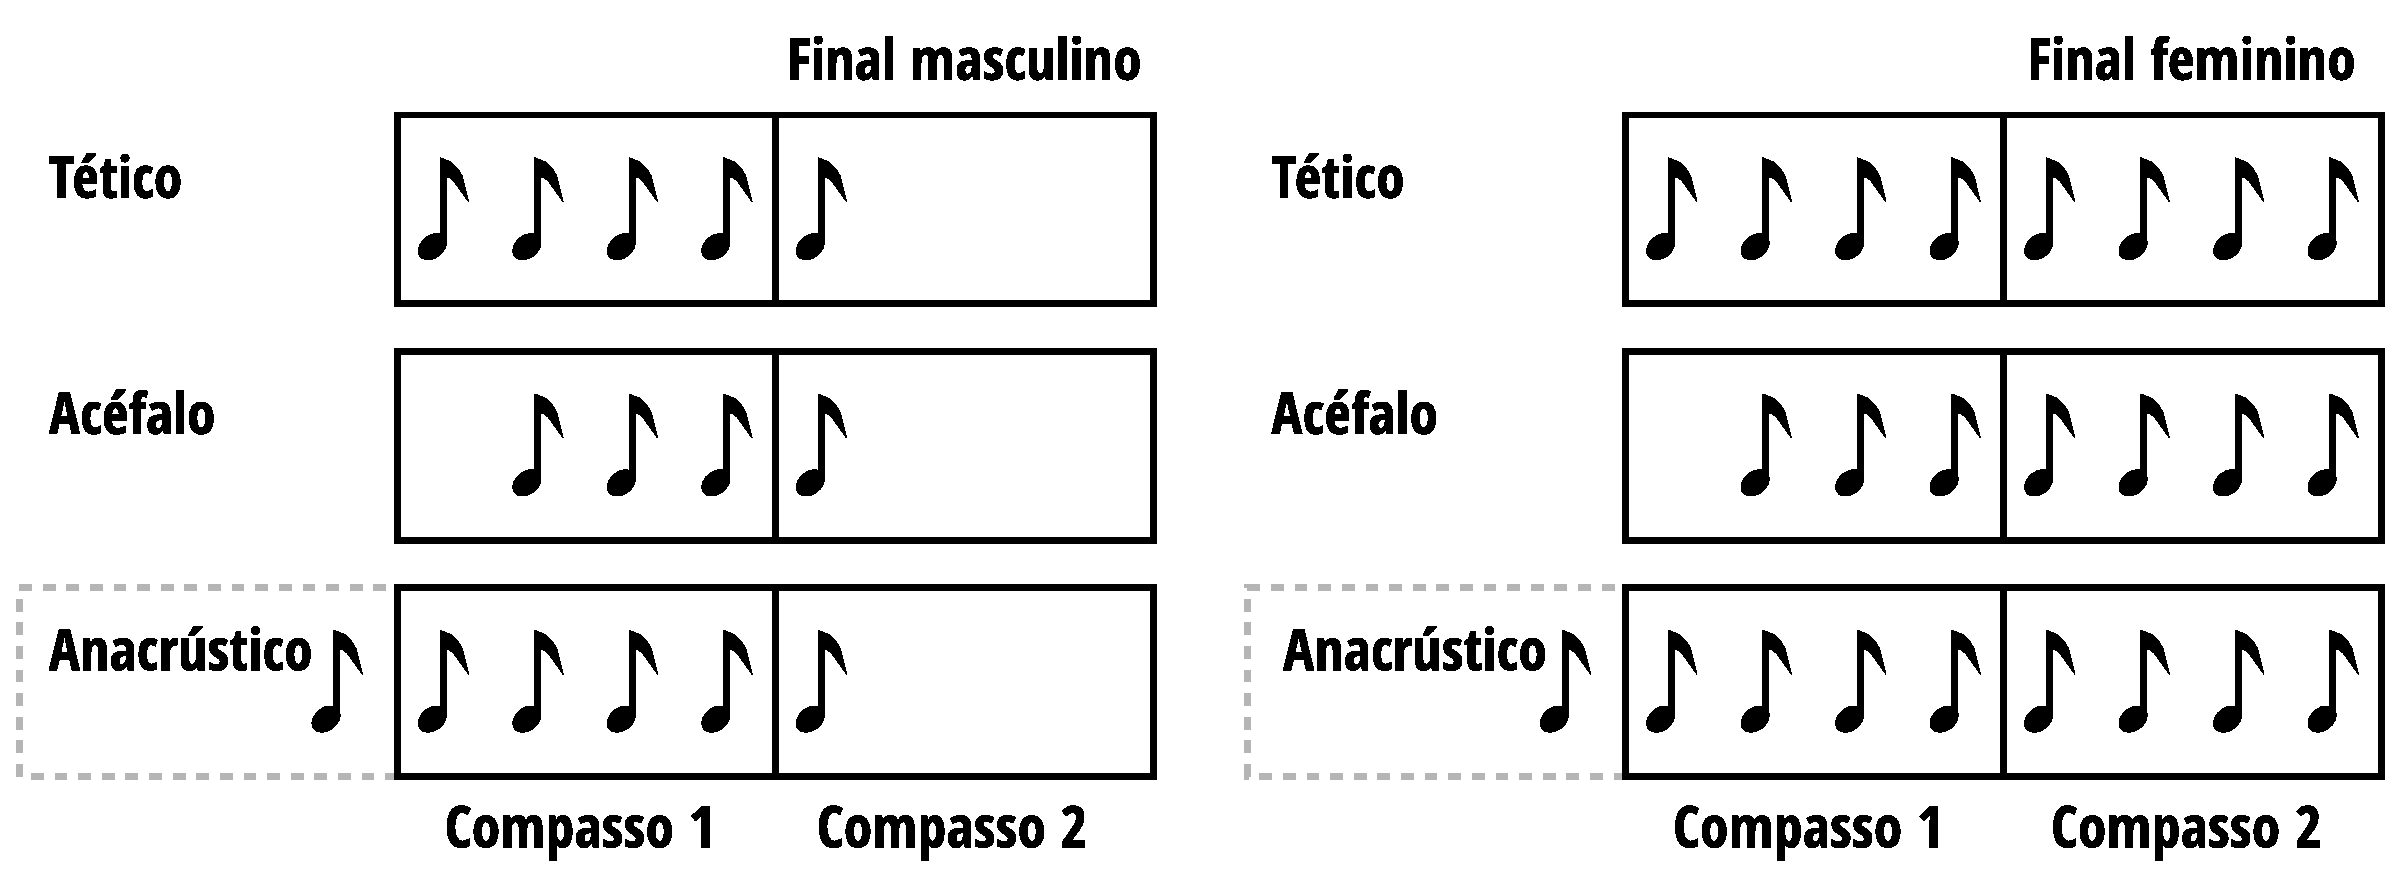
\includegraphics[width=\textwidth]{chapters/cap-musicalidade/contagemcompassosfrase.eps}
    \caption{Frases musicais com 2 compassos de comprimento.}
    \label{fig:contagemtemposfrase}
\end{figure}
É importante ressaltar que não importa a porção do compasso usado no final da frase,
pois este sempre é contado no comprimento;
mas isto não é assim no caso das notas no inicio,
pois o compasso que contem as anacruses não é computado.


\PRLsep{Detetando o inicio e o final de frase musical}


De forma geral, em músicas com textura \hyperref[subsec:monofonica]{\textbf{monofônica}} 
e \hyperref[subsec:homofonica]{\textbf{homofônica}} o acompanhamento percussivo ou harmônico 
se amolda à (única) linha melódica, 
pelo que identificar e seguir  as frases musicais pode ser mais simples no acompanhamento 
por ter uma caraterística regular e repetitiva.


%%%%%%%%%%%%%%%%%%%%%%%%%%%%%%%
\label{pos:detetandoiniciofrase}
Entre as dicas que podemos seguir para detetar o inicio de uma frase musical, encontramos que:
\begin{itemize}
\item Em musicas com uma única linha melódica, podemos detetar o inicio da frase musical,
analisando a letra ou sua melodia correspondente;
se apos uma pausa, escutamos primeiro uma nota em tempo forte (\hyperref[subsub:Tetico]{\textbf{tética}}),
então temos achado o inicio da frase e começamos a contagem desde esse compasso;
por outro lado se escutamos primeiro uma nota em tempo fraco,
devemos analisar se o inicio é \hyperref[subsub:anacrustica]{\textbf{anacrústico}} ou 
\hyperref[subsub:Acefalo]{\textbf{acéfalo}}; 
se o inicio é anacrústico, 
as notas antes do primeiro tempo forte e seu compasso são descartadas da contagem;
no caso contrario, estamos frente a um inicio acéfalo e o compasso sim é incluído na contagem. 
\item Existe geralmente, no primeiro tempo do primeiro compasso da frase, 
uma convergência de instrumentos de percussão, ou em geral do acompanhamento da melodia principal,
que provoca que este tempo forte seja percebido com maior \hyperref[sec:pos:Intensidade]{\textbf{intensidade}} 
que os outros tempos fortes da frase,
pelo que este tempo marca o inicio da contagem.
\item Na música \hyperref[subsec:homofonica]{\textbf{homofônica}} as harmonias de acompanhamento estão geralmente submetidas
à frase da melodia; assim, pela regularidade deste acompanhamento harmônico,
pode ser mais simples procurar o inicio da frase na harmonia.
\end{itemize}

%%%%%%%%%%%%%%%%%%%%%%%%%%%%%%%
\label{pos:detetandofinalfrase}
Entre as dicas que podemos seguir para detetar o final de uma frase musical, encontramos que:
\begin{itemize}
\item Geralmente entre o final de uma frase e o inicio de outra  
existe um tempo de espera maior que o visto nas notas regulares da frase.

\item Podemos detetar o final da frase se aprendemos a reconhecer os tipos de \hyperref[sec:Cadencia]{\textbf{Cadência}} 
vistas na Seção \ref{sec:Cadencia}.
\item Podemos prestar atenção ao \hyperref[ref:PontoCulminanteSuperior]{\textbf{ponto culminante superior}},
na frase musical dado que este indica que o final está próximo (ver Pag. \pageref{ref:PontoCulminanteSuperior}).
\item Podemos detetar o final da frase musical porque percebemos o enfases no inicio da seguinte frase.
\end{itemize}


\begin{example}[Músicas com frases de 4 compassos de comprimento:] ~
\label{ex:frasesde4compassos}
\begin{itemize}
\item ``Piston de gafieira'' de Billy Blanco.
\item ``Suingue de samba'' interpretado por Rogê.
\item ``Disritmia'' interpretado por Martinho da Vila.
\item ``Historia do samba'' interpretado por Joyce. % contando corporalmente é fácil de perceber.
\item ``impaciência'' interpretado por Luciana Mello.
%%%% quase regulares
\item ``Enfeitiçado'' interpretado por Aline Cardoso. 
Só tem uma frase de 3 compassos aproximadamente no meio da música.
\end{itemize}
\end{example}

\begin{comment}
\begin{tcbattention}
Podemos detetar intuitivamente o final de uma frase musical se 
interpretamos ela como se fosse uma frase falada (balbucio de uma criança) e 
percebemos nela o final de uma ideia, mais ideias na Seção \ref{subsec:fraseintuitivamente}.
\end{tcbattention}
\end{comment}

\begin{example}[Músicas com frases de 8 compassos de comprimento:] ~
\begin{itemize}
\item ``Altar particular'' interpretado por Maria Gadú. 
\item ``A cada dia que passa'' interpretado por Emílio Santiago.
\end{itemize}
\end{example}



\subsection{Separando frases intuitivamente}
\label{subsec:fraseintuitivamente}
Quando a música inclui letra é mais fácil distinguir intuitivamente  
onde inicia e finaliza uma frase,
pois nosso cérebro está treinado para perceber e processar a fala e sua estrutura;
reconhecendo automaticamente onde existem signos de pontuação como:
a virgula, o ponto e virgula, o ponto, o signo de admiração ou interrogação;
os quais descrevem finais de frases e nos indicam o tipo ou o proposito da frase e as que vem depois.

Este processamento automático não é exclusivo da fala num idioma em particular,
pois lembremos que quando escutamos a uma criança muito pequena tentando falar,
não conseguimos entender o significado dos seus balbucios, 
mas sim conseguimos separar as frases e identificar frases exclamativas e interrogativas,
frases afirmativas e suspensivas;
tudo isto sem precisar do conteúdo das palavras.

Assim, com um pouco de esforço e imaginação,
podemos supor que os sons de um instrumento musical 
são como balbucios de criança e podemos tentar extrair intuitivamente as frases musicais. 


\begin{example}[O discurso de ``la'']
\label{ex:discrusodela}
Usando unicamente a silaba ``la'', crie um discurso; por exemplo:
\begin{citando}%%
Lálala la lalá lá!\\
la lalá la lálala ...\\
la lalalá lála?\\
la lalá la lalalá.\\
\end{citando}%%
Logo proceda a ler acentuando, pausando e
executando signos de interrogação e admiração.

Perceba que o conteúdo das palavras não existe, 
porém pela expressividade na leitura é possível deduzir dos sonidos produzidos,
onde existem acentos, pausas, e signos de admiração ou interrogação.
\end{example}

\begin{example}
Na música ``Brasileirinho''  de Valdir Azevedo, 
ao tentar extrair as frases musicais, 
acontecerá o mesmo que com o discurso de ``la'' visto no Exemplo \ref{ex:discrusodela};
observaremos que:
\begin{itemize}
\item Teremos uma noção dos acentos na melodia e poderemos intuir, 
fazendo um levantamento estatístico,
em que tempo estará localizado o tempo forte. O analises será probabilístico,
pois na música existe a acentuação de tempos fracos (\hyperref[sec:contratempo]{\textbf{contratempos}}), 
pelo que se alguns tempos não cumprem com nossa predição podemos catalogar eles como contratempos.
\item Podemos perceber as pausas na melodia e deduzir que existe um final de \hyperref[sec:Frase]{\textbf{frase}} musical ou intuir o uso de uma \hyperref[fig:Cesura]{\textbf{cesura}}.
\item Também podemos perceber diferentes formas de finalizar uma frase, 
que na linguagem falada associaríamos com o uso ou não de signos de admiração e exclamação;
no âmbito da música, temos algo similar mediante o uso das \hyperref[sec:Cadencia]{\textbf{cadências}}.
Assim, cada tipo de cadência nos dará uma ideia diferente da função que cumpre a frase no discurso da peça musical 
e se existirá ou não uma frase de resposta.
\end{itemize}
\end{example}

\section{Percepção do breque na música}
\label{sec:percepcionbreak}
\index{Musicalidade!Breque}

Uma habilidade muito comentada quando uma pessoa inicia o estudo da musicalidade 
é a capacidade de distinguir as interrupções na música, 
também chamadas breques (deformação do termo ``break'' em inglês) ou paradinhas.

É importante aclarar que as pausas acontecem o tempo todo na  música,
porém quando mencionamos aos breques, 
em geral as pessoas se referem às pausas que acontecem ao final de uma frase musical 
e que além de marcar o final desta numa linha melódica,
acontecem numa pausa dos instrumentos de acompanhamento da música.
Muitas vesses poderemos observar um tempo de espera maior no breque que entre duas frases consecutivas regulares.
Outra caraterística dos breques é que comumente está pausa é preenchida por uma melodia auxiliar 
que funciona como resposta para a frase anterior e que da uma ideia ao ouvinte de quando o breque terminará.
Na música \hyperref[subsec:monofonica]{\textbf{monofônica}} e \hyperref[subsec:homofonica]{\textbf{homofônica}} 
o breque geralmente pode ser percebido pela pausa do acompanhamento percussivo principal;
já na música \hyperref[subsec:polifonica]{\textbf{polifônica}} o breque pode ser total,
ou só incluir a uma melodia dando entrada a outra voz que pode ou não levar acompanhamento.
\begin{definition}[Breque]
\label{def:breakingoff}  
\index{Musicalidade!Breque}
Também chamado ``Abruptio'' ou ``a breaking-off''. 
Esta é uma parada repentina numa melodia que acontece antes de chegar ao verdadeiro final da música, 
de modo que a peça continua após a pausa \cite[pp. 5]{baker1895dictionary}

Este recurso é geralmente utilizado para agregar mais emoção,
ou para dar uma sensação de antecipação para a nova seção da música. 

A pausa pode ser total ou pode incluir um pequeno solo melódico ou percussivo, 
também existe a possibilidade de combinar ambas opções.
%Definição de abruptio e outras pausas \cite{villavicencio2011retorica}.

\end{definition}

\begin{definition}[Break]
\index{Musicalidade!Break}
É o ponto de junção na qualidade das vozes de tenor, soprano e alto
ou da voz de cabeça e a de tórax;  
em geral pode entender-se como o ponto no qual um registro de voz ou instrumento passa para outro 
\cite[pp. 63]{stainer2009dictionary} \cite[pp. 31]{baker1895dictionary}.
\end{definition}

Com estas descrições do breque na música, 
podemos inferir que se sabemos detetar o 
\hyperref[pos:detetandofinalfrase]{\textbf{final de uma frase musical}}\footnote{A
detecção do final de uma frase musical foi explicado na Pag. \pageref{pos:detetandofinalfrase}.},
então provavelmente saberemos detetar os breques na música.
Porém existem particularidades do breque
que nós ajudarão a predizê-los mais facilmente, como:
\begin{itemize}
%%%%%
\item \hyperref[sec:tensionrelease]{\textbf{Tensão e relaxação:}} Como vimos na Seção \ref{sec:tensionrelease},
existe na música uma dinâmica continua de tensão e relaxação 
que é intuitivamente perceptível se prestamos um pouco atenção à música.
Esta caraterística nos será muito útil, 
pois os breques geralmente são anunciados por uma acumulação acentuada da tensão,
chegando ao ponto de não ter um possível retorno amável à relaxação, 
pelo que a única saída esperada pelo ouvinte é que a música ``estoure'';
ou seja, que tenha um breque.
Para mais detalhes sobre indicadores que ajudam a perceber tensão na música, ir a Tabela \ref{tab:tensionrelease1}.
Exemplos do uso da tensão e relaxação musical na dança podem ser vistos na Seção \ref{sec:musicalidadetensionrelease}.
%%%%%
\item \textbf{Atenção ao tempo forte:} A maioria de breques na música acontecem no tempo forte,
isto é devido a que as frases com \hyperref[subsubsec:finalmasculino]{\textbf{final masculino}} 
tem uma maior sensação de conclusão e tendem a ser mais empolgantes que 
\hyperref[subsubsec:finalfemenino]{\textbf{finais femininos}} que dão uma sensação mais reflexiva, 
suspensiva ou interrogativa, dependendo da cadência.
Os compositores ao criar um breque na música geralmente procuram ter uma pausa conclusiva, explosiva e contundente,
pelo menos em musicas alegres.
Assim, é importante estar atentos ao tempo forte quando, por exemplo, 
pelo acumulo de tensão sabemos que um breque está próximo.
\begin{example}[Breques em músicas (final masculino e/ou com sincopados):]~
\label{ex:breakmasculinos}
\begin{itemize}
\item ``Baile no Elite'' interpretado por Casuarina.
\item ``Cabide'' interpretado por Ana Carolina e Luiz Melodia.
\item ``Reunião de Bacana (Se gritar pega ladrão)'' interpretado pelo grupo Exporta Samba.
\item ``Tiro ao Álvaro'' interpretado por Elis Regina e Adoniran Barbosa. 
\item ``A voz do morro'' interpretado por Diogo Nogueira.
\end{itemize}
\end{example}

%%%%%
\item \textbf{Predizer na melodia e seguir o acompanhamento:}
Como falamos anteriormente a pausa geralmente acontece no tempo forte,
mas é possível achar pausas que acontecem no tempo fraco. 
Pelo que em algumas ocasiones teremos duvidas em reconhecer ou predizer em que tempo acabará a frase,
como é visto no Exemplo \ref{ex:breakforte1}.
\begin{example}
\label{ex:breakforte1}
Na música ``Reunião de Bacana (Se gritar pega ladrão)'' interpretado pelo grupo Exporta Samba,
existe um breque no final da frase: ``Para ser rou\textbf{ba}do...''
na qual a sílaba tônica ``ba'' se percebe próxima ao tempo forte, 
pelo que poderíamos supor que a frase termina em tempo fraco na sílaba ``do'';
porém o que nos resolve esta duvida é o acompanhamento percussivo, 
que claramente finaliza com uma nota em tempo forte.
Assim podemos especular que o breque aconteceu no tempo forte
no final da frase ``Para ser rou\textbf{ba}do...''.
\end{example}
Assim, para evitar estas duvidas na conjetura e qualificação do tipo de breque,
é melhor predizer este usando a melodia principal 
e classificar-lho usando a posição das notas finais do acompanhamento harmônico ou percussivo.
%%%%%
\item \hyperref[ref:PontoCulminanteSuperior]{\textbf{Ponto culminante superior:}} 
A nota mais aguda da frase musical\footnote{O 
ponto culminante superior foi mencionado na Pag. \pageref{ref:PontoCulminanteSuperior}.} 
é um bom indicador para detetar que um final de frase musical está próximo; 
consequentemente, se por outros fatores como acumulação de tensão,
sabemos que estamos perto de um breque, escutar esta nota mais aguda acentuará nossa certeza ao predizer 
a proximidade deste evento.

%\item Podemos detetar o final de uma frase pois, 
%ao ser interpretada como se fosse uma frase falada, 
%percebemos que uma ideia está chegando a seu final.

%\item Podemos aprender a reconhecer os tipos de \hyperref[sec:Cadencia]{\textbf{Cadência}},
%vistas na Seção \ref{sec:Cadencia}.
\end{itemize}



\begin{example}[Breques em músicas com final feminino]~
\label{ex:breakfeminino}
\begin{itemize}
\item ``Amanhã é sábado'' interpretado por Roberta Sá. 
O primeiro breque acontece com um final de frase feminino.
\end{itemize}
\end{example}

\begin{example}[Breques em músicas com final sincopado]~
\label{ex:breaksincopados}
\begin{itemize}
\item ``Eu sou a marrom'' interpretado por Alcione.
\item ``Logo agora'' interpretado por Emílio Santiago.
\end{itemize}
\end{example}




%\section{Reconhecendo o tom}
% \cite[pp. 116]{alves2004teoria}

